

\begin{definition}[Matching logic syntax and semantics]\label{def:matchinglogic}
We define the matching logic syntax and semantics as follows.
\begin{enumerate}
    \item A matching logic \emph{signature} $\mathbf{\Sigma} = (\Sigma, \mathit{Var})$ is a many-sorted algebraic signature $\Sigma$ together with a sort-wise infinite set of variables $\mathit{Var}$.
    \item Let $T_{\Sigma}(\mathit{Var})$ denote the free $\Sigma$-algebra of terms with variables 
          in $\mathit{Var}$.
          Let $T_{\Sigma, s}(\mathit{Var})$ denote the set of $\Sigma$-terms (with variables in $\mathit{Var})$ of sort $s$.
    \item Let $\mathcal{T}$ be a $\Sigma$-algebra, and $f$ be a symbol from $\Sigma$.
          We use the notation $\mathcal{T}_f$ to denote the interpretation of $f$ in $\mathcal{T}$.
    \item A function $\rho : \mathit{Var} \to \mathcal{T}$, where $\mathcal{T}$ is a $\Sigma$-algebra,
          extends uniquely (in the usual way) to a $\Sigma$-algebra morphism
          $\rho : T_{\Sigma}(\mathit{Var}) \to \mathcal{T}$.
    \item The set of \emph{nullary predicate symbols} $P_\epsilon((\Sigma, \mathit{Var}))$
          (or just $P_\epsilon$ if $(\Sigma, \mathit{Var})$ is known from the context) is
          defined to contain exactly terms $\phi \in T_{\Sigma, s}(\mathit{Var})$.
    \item A matching logic $(\Sigma, \mathit{Var})$-formula (aka $(\Sigma, \mathit{Var})$-\emph{pattern})
          of sort $s$
          is a $(\Sigma, P_\epsilon)-\FOLeq$ formula (that is, a $\FOLeq$ formula where function symbols are
          exactly symbols from $\Sigma$, and where nullary predicate symbols are exactly
          terms $\phi \in T_{\Sigma, s}(\mathit{Var})$, without any $k$-ary predicate symbols for $k > 0$).
          We let $\Pattern(\mathbf{\Sigma})$ (or just $\Pattern$ when $\mathbf{\Sigma}$ is known from the context)
          denote the set of all $\mathbf{\Sigma}$-patterns.
    \item Let $\mathit{FV}(\varphi)$ denote the set of all free variables of $\varphi$.
    \item A matching logic pattern is \emph{structureless} if it contains
          no terms $\phi \in T_{\Sigma, s}(\mathit{Var})$ used as predicates.
    \item A \emph{constrained term} is a pattern of the form $\phi \land P$,
          where $\phi \in T_{\Sigma, s}(\mathit{Var})$ and $P$ a structureless pattern.
    \item A matching logic $\Sigma$-\emph{model} $\mathcal{T}$ is a $\Sigma$-algebra with non-empty carrier sets.
    \item A matching logic \emph{semantics} is given by means of
          the satisfaction relation $\vDash_{\ML}$ between a matching logic $\Sigma$-model,
          a model element, and a valuation,
          defined inductively as
          \begin{itemize}
              \item $(\mathcal{T}, \gamma, \rho) \vDash \phi$ iff $\gamma = \rho(\phi)$, where $\phi \in T_{\Sigma, s}(\mathit{Var})$;
              \item $(\mathcal{T}, \gamma, \rho) \vDash \varphi_1 \land \varphi_2$ iff
                $(\mathcal{T}, \gamma, \rho) \vDash \varphi_1$ and
                $(\mathcal{T}, \gamma, \rho) \vDash \varphi_2$;
              \item $(\mathcal{T}, \gamma, \rho) \vDash \neg \varphi$ iff
                $(\mathcal{T}, \gamma, \rho) \not\vDash \varphi$;
              \item $(\mathcal{T}, \gamma, \rho) \vDash \exists x : s.\, \varphi$ iff
                $(\mathcal{T}, \gamma, \rho^\prime) \vDash \varphi$ for some $\rho^\prime$ such that
                $\rho^\prime(y) = \rho(y)$ for all $y \in \mathit{Var} \setminus \{ x \}$
                and $\rho^\prime(x) \in \mathcal{T}_s$;
          \end{itemize}
          
\end{enumerate}

\end{definition}


\begin{lemma}\label{lem:structurelessSemantics}
Let $\mathcal{T}$ be a matching logic $\Sigma$-model, $\gamma,\gamma^\prime \in \mathcal{T}$ model elements,
and $\rho$ a $\mathcal{T}$-valuation. Then for any structureless pattern $P$,
\begin{equation*}
    (\mathcal{T}, \gamma, \rho) \vDash P \iff (\mathcal{T}, \gamma^\prime, \rho) \vDash P \, .
\end{equation*}
Therefore, when $P$ is structureless, we may sometimes write $(\mathcal{T}, \rho) \vDash P$ to mean that 
$(\mathcal{T}, \gamma, \rho) \vDash P$ for \emph{some} $\gamma \in \mathcal{T}$.
\end{lemma}
\begin{proof}[Proof of \Cref{lem:structurelessSemantics}]
Let $P$ be a structureless pattern.
We perform induction on $P$.
If $P = \phi$, we get contradiction with the assumption that $P$ is structureless;
therefore, the conclusion holds by \emph{ex falso quodlibet}.
Other cases follow from the induction hypotheses.
\end{proof}

\begin{lemma}\label{lem:unusedVariables}
    Let $\mathcal{T}$ be a matching logic model, $\gamma$ an element of this model,
    and $\varphi$ a pattern.
    Then for any two $\mathcal{T}$-valuations $\rho,\rho^\prime$
    satisfying $\rho^\prime(y) = \rho(y)$ for any $y \in \mathit{FV}(\varphi)$,
    \begin{equation*}
        (\mathcal{T}, \gamma, \rho) \vDash \varphi \iff (\mathcal{T}, \gamma, \rho^\prime) \vDash \varphi \, .
    \end{equation*}
\end{lemma}
\begin{proof}
Admitted.
\end{proof}




\begin{definition}[\cite{StefanescuCMMSR19}]
    Given a  matching logic $(\Sigma, \mathit{Var})$-formula $\varphi$ of sort $\mathit{Cfg}$,
    and a fresh (with respect to $\varphi$) variable $\square$ of sort $\mathit{Cfg}$,
    we let $\varphi^\square$ denote the $\FOLeq$ formula formed from $\varphi$ by replacing
    nullary predicate symbols $\phi \in T_{\Sigma, \mathit{Cfg}}(\mathit{Var})$
    with equalities $\square = \phi$.
    Given a matching logic $(\Sigma, \mathit{Var})$-model $\mathcal{T}$, a $\mathcal{T}$-valuation $\rho$,
    and an element $\gamma \in \Tcfg$,
    we let the $\mathcal{T}$-valuation $\rho^\gamma$ be such that $\rho^\gamma(\square) = \gamma$,
    and $\rho^\gamma(x) = \rho(x)$ for $x \not = \square$.
\end{definition}

\begin{lemma}[\cite{StefanescuCMMSR19}]\label{lem:patternToFOLSemantics}
    Whenever $\square$ is fresh in $\varphi$, we have
    \begin{equation*}
        (\mathcal{T}, \gamma, \rho) \vDash \varphi \iff (\mathcal{T}, \rho^\gamma) \vDash \varphi^\square
    \end{equation*}    
\end{lemma}

\begin{definition}[\cite{StefanescuCMMSR19,RosuS12oopsla}]\label{def:basics}
We define reachability-logic signatures, rules, and systems as follows.
\begin{enumerate}
    \item A reachability-logic \emph{signature} is a pair $(\mathbf{\Sigma}, \mathit{Cfg})$,
          where $\mathbf{\Sigma}$ is a matching logic signature and $\mathit{Cfg}$ is a sort from $\mathbf{\Sigma}$.
          
    \item A \emph{one-path reachability rule} over reachability logic signature $(\mathbf{\Sigma}, \mathit{Cfg})$        is a pair $\varphi \Rightarrow^\exists \varphi^\prime$,
          where $\varphi$ and $\varphi^\prime$
          are $\mathbf{\Sigma}$-patterns (which can have free variables) of sort $\mathit{Cfg}$.
          
    \item A \emph{reachability system} over a reachability-logic signature $((\Sigma, \mathit{Var}), \mathit{Cfg})$
          is a pair $\mathcal{S} = (\mathcal{T}, S)$, where $\mathcal{T}$ is a $\Sigma$-algebra
          and $S$ is a set of reachability rules over $((\Sigma, \mathit{Var}), \mathit{Cfg})$.
          
    \item A rule $\varphi \Rightarrow^\exists \varphi^\prime$ over $((\Sigma, \mathit{Var}), \mathit{Cfg})$
          is \emph{weakly well-defined}
          with respect to $\Sigma$-algebra $\mathcal{T}$
          iff
          for any $\gamma \in \Tcfg$ and $\rho : \Var \to \mathcal{T}$
          with $(\gamma, \rho) \vDash \varphi$,
          there exists $\gamma^\prime \in \Tcfg$ with $(\gamma^\prime , \rho) \vDash \varphi^\prime$.
          
    \item A reachability system $\mathcal{S}$ is \emph{weakly well-defined} iff each its rule is weakly     
          well-defined.
          
    \item A reachability system $\mathcal{S} = (\mathcal{T}, S)$ over $((\Sigma, \mathit{Var}), \mathit{Cfg})$ induces
          a \emph{transition system} \\
          $(\Tcfg , \Rightarrow_{\mathcal{S}})$,
          where $\gamma \Rightarrow_{\mathcal{S}} \gamma^\prime$
          for $\gamma, \gamma^\prime \in \Tcfg$
          iff there is some rule \\ $\varphi \Rightarrow^\exists \varphi^\prime \in S$
          and some valuation $\rho : \Var \to \mathcal{T}$ with $(\gamma, \rho) \vDash \varphi$
          and $(\gamma^\prime , \rho) \vDash \varphi^\prime$.

    \item A reachability system $(\mathcal{T}, S)$ is \emph{deterministic} iff the induced transition system
          is deterministic.
          
    \item A reachability system $(\mathcal{T}, S)$ is \emph{$\epsilon$-free}
          iff for any two configurations $\sigma, \sigma^\prime \in \mathcal{T}_{\mathit{Cfg}}$, if
          $\sigma \Rightarrow_{\mathcal{S}} \sigma^\prime$, then $\sigma \not = \sigma^\prime$.

    \item A configuration $\gamma \in \Tcfg$ \emph{terminates} in $(\Tcfg , \Rightarrow_{\mathcal{S}})$
          iff there is no infinite $\Rightarrow_{\mathcal{S}})$-sequence starting with $\gamma$.
          
    \item A \emph{$\Rightarrow_{\mathcal{S}}$-path} is a finite
          sequence $\gamma_0 \Rightarrow_{\mathcal{S}} \gamma_1 \Rightarrow_{\mathcal{S}} \ldots
          \Rightarrow_{\mathcal{S}} \gamma_n$
          with $\gamma_0,\ldots,\gamma_n \in \Tcfg$.
          
    \item A $\Rightarrow_{\mathcal{S}}$-path is \emph{complete}
          iff it is not a strict prefix of any
          other $\Rightarrow_{\mathcal{S}}$-path.

    \item \label{def:oprlSemantics}
          A one-path reachability rule $\varphi \Rightarrow^\exists \varphi^\prime$ is \emph{satisfied}
          in a reachability system $\mathcal{S} = (\mathcal{T}, S)$,
          written $\mathcal{S} \vDash_\RL \varphi \Rightarrow^\exists \varphi^\prime$,
          iff for every $\gamma \in \Tcfg$
          such that $\gamma$ terminates in $(\Tcfg, \Rightarrow_{\mathcal{S}})$
          and for any valuation $\rho : \Var \to \mathcal{T}$
          such that $(\gamma, \rho) \vDash \varphi$,
          there exists some $\gamma^\prime \in \Tcfg$
          such that
          $\gamma \Rightarrow^{*}_{\mathcal{S}} \gamma^\prime$
          and $(\gamma^\prime, \rho) \vDash \varphi^\prime$.
          
          
%    \item An \emph{all-path reachability rule} is a pair
%        $\varphi \Rightarrow^\forall \varphi^\prime$ of patterns $\varphi$ and $\varphi^\prime$.
%    
%    \item \label{def:aprlSemantics}
%          An all-path reachability rule $\varphi \Rightarrow^\forall \varphi^\prime$ is \emph{satisfied},
%          written $\mathcal{S} \vDash_\RL \varphi \Rightarrow^\forall \varphi^\prime$,
%          iff for all complete $\Rightarrow_{\mathcal{S}}$-paths $\tau$
%          starting with $\gamma \in \Tcfg$ and for all $\rho : \Var \to \mathcal{T}$
%          such that $(\gamma, \rho) \vDash \varphi$,
%          there exists some $\gamma^\prime \in \tau$
%          such that $(\gamma^\prime, \rho) \vDash \varphi^\prime$.
\end{enumerate}

\end{definition}

\begin{definition}[CRL Syntax]\label{def:opCRLSyntax}
    We define the syntax of Cartesian Reachability logic as follows:
    \begin{itemize}
        \item 
    A \emph{list-pattern} has the shape $[\varphi_1,\ldots,\varphi_k]$,
              where each $\varphi_j$ (for $j \in \{ 1, \ldots, k \} $) is a matching logic pattern.
        \item
              A \emph{constrained list-pattern (CLP)} is a conjunction $\Psi_0 \land P$
              of a list-pattern $\Psi_0$ and a structureless pattern $P$.
        \item
              An \emph{existentially-quantified constrained list-pattern (ECLP)} has the form
              $\exists \vec{Y}.\, \Psi$, where $\Psi$ is a CLP and $\vec{Y}$ is a (possibly empty) list of variables.
        \item
              A \emph{One-Path Cartesian reachability claim of arity $k$} has the shape
              $\Phi \Rightarrow^{c\exists} \Psi$,
              where $\Phi$ is a CLP and $\Psi$ is an ECLP.
    \end{itemize}
\end{definition}    

\begin{definition}\label{def:starextension}
We translate a language semantics into a semantics for lists of configurations as follows.
\begin{enumerate}
    \item Let $((\Sigma, \mathit{Var}), \mathit{Cfg})$ be a reachability-logic signature.
          Then $((\Sigma, \mathit{Var}^*), \mathit{Cfg})^*$ = $((\Sigma^*, \mathit{Var}^*), \mathit{Cfg}^*)$,
          where
          \begin{enumerate}
              \item $\Sigma^* = \Sigma \cup \{ \mathit{cfgitem}, \mathit{cfgconcat}, \mathit{cfgheat}, \mathit{cfgnil} \}$
              \item $\mathit{Cfg}^*$ is a fresh sort (representing the sort of lists of configurations);
              \item $\mathit{Var}^* = \mathit{Var} \cup \mathit{Var}_{\mathit{Cfg}^*}$,
              where $\mathit{Var}_{\mathit{Cfg}^*}$ is an infinite set of variables of sort $\mathit{Cfg}^*$,
              distinct from varibles in $\mathit{Var}$;
              \item $\mathit{cfgitem}$ a fresh symbol of sort $\mathit{Cfg} \to \mathit{Cfg}^*$;
              \item $\mathit{cfgnil}$ a fresh symbol of sort $\mathit{Cfg}^*$;
              \item $\mathit{cfgconcat}$ a fresh symbol of sort $\mathit{Cfg}^* \times \mathit{Cfg}^* \to \mathit{Cfg}^*$; and
              \item $\mathit{cfgheat}$ is a fresh symbol of sort $\mathit{Cfg}^* \times \mathit{Cfg} \times \mathit{Cfg}^* \to \mathit{Cfg}^*$.
          \end{enumerate}
    \item Let $S$ be a set of reachability rules over $(\mathbf{\Sigma}, \mathit{Cfg})$.
          We generate a set of reachability rules $S^*$ over $(\mathbf{\Sigma}, \mathit{Cfg})^*$
          by
          \begin{enumerate}
              \item defining a function $\mathit{heat} : \mathit{Var} \times \Pattern \times \mathit{Var} \to \Pattern$ by
              \begin{align*}
                  \mathit{heat}(L, \phi \land P, R)
                  = \mathit{cfgheat}(L, \phi, R) \land P
              \end{align*}
              \item setting
              \begin{align*}
              S^* = \{ \mathit{heat}(L, \varphi, R) \Rightarrow^\exists \mathit{heat}(L, \varphi^\prime, R)
              \mid  ( \varphi \Rightarrow^\exists \varphi^\prime ) \in S \} \, ,
            \end{align*}
                          where $L,R$ are distinct fresh variables (not occurring in any rule in $S$).
          \end{enumerate}
    \item Let $(\Sigma, \mathit{Var})$ be a matching logic signature, and let $\mathcal{T}$ be a configuration model; that is, a $\Sigma$-algebra.
          We generate a $\Sigma^*$-algebra $\mathcal{T}*$, which interprets all sorts and symbols from
          $\Sigma$ as in $\mathcal{T}$, and in addition interprets
          \begin{enumerate}
              \item the sort $\mathit{Cfg}*$ as the set of all finite lists
              $[c_1;\ldots;c_n]$ for $n \in \mathbb{N}$, where $c_i$ is an element of sort $\mathit{Cfg}$
              for any $0 \leq i \leq n$;
              \item the symbol $\mathit{cfgitem}$ as the function $\lambda c.\, [c]$;
              \item the symbol $\mathit{cfgnil}$ as the empty list ($[]$);
              \item the symbol $\mathit{cfgconcat}$ as the function $\lambda l_1,l_2.\, l_1 \texttt{++} l_2$,
                where $\texttt{++}$ is list concatenation; and
              \item the symbol $\mathit{cfgheat}$ as the function
                $\lambda l_1, c, l_2.\, l_1 \texttt{++} [c] \texttt{++} l_2$.
          \end{enumerate}

    \item Let $(\Sigma, \mathit{Var})$ be a matching logic signature, let $\mathcal{T}$ be a configuration model,
        and let $\rho$ be a $\mathcal{T}$-valuation.
        We define a $\mathcal{T}^*$-valuation $\rho^*$ by letting $\rho^*(v) = \rho(v)$ for any $v \in \mathit{Var}$,
        and letting $\rho^*(v) = a$, where $a$ is some arbitrary element of sort $\mathit{Cfg}^*$, for
        any variable $v$ of sort $\mathit{Cfg}^*$.
          
    \item Let $\mathcal{S} = (\mathcal{T}, S)$ be a reachability system over $(\Sigma, \mathit{Cfg})$.
          We generate a reachability system $\mathcal{S}^*$ over $(\Sigma, \mathit{Cfg})^*$
          by setting $\mathcal{S}^* = (\mathcal{T}^*, S^*)$.
\end{enumerate}
\end{definition}

\begin{lemma}\label{lem:rhoStarOfPi}
    Let $(\Sigma, \mathit{Var})$ be a matching logic signature, $\mathcal{T}$ be a configuration model,
    and $\rho$ be a $\mathcal{T}$-valuation. Then for any basic $(\Sigma, \mathit{Var})$-pattern $\pi$,
    \begin{equation}
        \rho^*(\pi) = \rho(\pi) \, .
    \end{equation}
\end{lemma}

\begin{proof}[Proof of \Cref{lem:rhoStarOfPi}]
    By induction on the term $\pi$.
    \begin{itemize}
        \item $\pi = v$ for $v \in \mathit{Var}$ - follows from the definition of $\rho^*$.
        \item $\pi = f(\pi_1, \ldots, \pi_k)$ - we have $\rho(\pi_i) = \rho^*(\pi_i)$ for any $i \in \{ 1, \ldots, k \}$
              by the induction hypothesis.
              Then
              \begin{align*}
                  \rho^*(f(\pi_1, \ldots, \pi_k)) 
                  = & {\mathcal{T}^*}_f(\rho^*(\pi_1), \ldots, \rho^*(\pi_k)) \\
                  = & {\mathcal{T}^*}_f(\rho(\pi_1), \ldots, \rho(\pi_k)) \\
                  = & \mathcal{T}_f(\rho(\pi_1), \ldots, \rho(\pi_k)) \\
                  = & \rho(f(\pi_1, \ldots, \pi_k))
              \end{align*}
              where the second-to-last equality holds by definition of $\mathcal{T}^*$.
    \end{itemize}
\end{proof}

\begin{lemma}\label{lem:starConservative}
    The star extension on matching logic models is conservative, in the following sense.
    For any $\Sigma$-model $\mathcal{T}$, any $\mathcal{T}$-valuation $\rho$,
    any $\Sigma$-sort $s$,
    any $\gamma \in \mathcal{T}_s$,
    and any matching logic $s$-pattern $\varphi$,
    \begin{equation*}
        (\mathcal{T}, \gamma, \rho) \vDash \varphi \iff (\mathcal{T}^*, \gamma, \rho^*) \vDash \varphi
    \end{equation*}
\end{lemma}

\begin{proof}[Proof of \Cref{lem:starConservative}]
By induction on $\varphi$.
\begin{itemize}
    \item $\varphi \equiv \pi$, where $\pi$ is a basic pattern (of sort $s$) - follows from \Cref{lem:rhoStarOfPi}.
    \item $\varphi \equiv \varphi_1 \land \varphi_2$ - follows from the induction hypothesis.
    \item $\varphi \equiv \neg \varphi^\prime$ - follows from the induction hypothesis.
    \item $\varphi \equiv \exists x : s^\prime.\, \varphi^\prime$. We have
    $ (\mathcal{T}^*, \gamma, \rho^\prime) \vDash \exists x : s^\prime.\, \varphi^\prime $
    if and only if (by definition of $\vDash$)
    there exists some valuation ${\rho^*}^\prime : \mathit{Var} \to \mathcal{T}^*$ such that
    $(\mathcal{T}^*, \gamma, {\rho^*}^\prime) \vDash \varphi^\prime$
    and ${\rho^*}^\prime(x) \in \mathcal{T}^*_{s^\prime}$\traian{you need to use $s'$ here and in the following.}
    and ${\rho^*}^\prime(y) = \rho^*(y)$ for all $y \in \mathit{Var} \setminus \{ x \}$.
    This holds if and only if
    there exists some valuation $\rho^{\prime} : \mathit{Var} \to \mathcal{T}$ such that
    $(\mathcal{T}^*, \gamma, {\rho^{\prime}}^*) \vDash \varphi^\prime$
    and ${\rho^{\prime}}^*(x) \in \mathcal{T}^*_s$
    and ${\rho^{\prime}}^*(y) = \rho^*(y)$ for all $y \in \mathit{Var} \setminus \{ x \}$:
    one implication follows by letting ${\rho^*}^\prime := \rho^{\prime}$;
    for the other implication, we let $\rho^{\prime}(v) := {\rho^*}^\prime(v)$ for all $v \in \mathit{Var}$,
    and by the definition of star, we have ${\rho^{\prime}}^*(v) = {\rho^*}^\prime(v)$, from which the rest follows.
    Next, by the induction hypothesis, this holds if and only if
    there exists some valuation $\rho^{\prime} : \mathit{Var} \to \mathcal{T}$ such that
    $(\mathcal{T}, \gamma, {\rho^{\prime}}) \vDash \varphi^\prime$
    and ${\rho^{\prime}}^*(x) \in \mathcal{T}^*_s$
    and ${\rho^{\prime}}^*(y) = \rho^*(y)$ for all $y \in \mathit{Var} \setminus \{ x \}$.
    Next, by the definition of ${\rho^\prime}^*$ and $\rho^*$, this holds if and only if
    there exists some valuation $\rho^{\prime} : \mathit{Var} \to \mathcal{T}$ such that
    $(\mathcal{T}, \gamma, {\rho^{\prime}}) \vDash \varphi^\prime$
    and ${\rho^{\prime}}(x) \in \mathcal{T}^*_s$
    and ${\rho^{\prime}}(y) = \rho(y)$ for all $y \in \mathit{Var} \setminus \{ x \}$.
    But since the star extensions interprets all sorts from $\Sigma$ as in the original model
    (that is, $\mathcal{T}^*_s = \mathcal{T}_s$),
    this is equivalent to the semantics of $(\mathcal{T}, \gamma, \rho) \vDash \exists x:s^\prime.\, \varphi^\prime$,
    which is what we wanted to prove.

    Alternate attempt:
    The induction hypothesis is: for any $\mathcal{T}$, $\gamma$, $\rho$, 
        $$(\mathcal{T}, \gamma, \rho) \vDash \varphi' \iff (\mathcal{T}^*, \gamma, \rho^\ast) \vDash \varphi'$$
    We want to prove that for any $\mathcal{T}$, $\gamma$, $\rho$, 
        $$(\mathcal{T}, \gamma, \rho) \vDash \exists x:s'. \varphi' \iff (\mathcal{T}^*, \gamma, \rho^\ast) \vDash \exists x:s'.\varphi'$$
    
    First, let us prove the left-to-right implication.
    The left-hand-side of the claim is equivalent with
    $$\exists \rho'. (\forall y. y \neq x \to \rho'(y) = \rho(y)) \wedge (T, \gamma, \rho') \vDash \varphi'$$
    From the induction hypothesis, this is further equivalent with
    $$\exists \rho'. (\forall y. y \neq x \to \rho'(y) = \rho(y)) \wedge (T^\ast, \gamma, {\rho'}^\ast) \vDash \varphi'$$
    
    Since $\forall y. y \neq x \to {\rho'}^\ast(y) = \rho'(y) = \rho(y) = \rho^\ast(y)$, we deduce $(\mathcal{T}^*, \gamma, \rho^\ast) \vDash \exists x:s'.\varphi'$.
    
    Conversely, the right-hand-side of the claim is equivalent with
    $$\exists \rho''. (\forall y. y \neq x \to \rho'(y) = \rho\ast(y)) \wedge (T^\ast, \gamma, \rho'') \vDash \varphi'$$
    Let $\rho'$ be defined by $\rho'(y) = \rho(y)$ if $y\neq x$ and $\rho'(x) = \rho''(x)$. Then it is
    easy to see that ${\rho'}^\ast = \rho''$, whence by the induction hypothesis we obtain that
    $(T, \gamma, \rho') \vDash \varphi'$, and by the definition of $\rho'$, $(T, \gamma, \rho) \vDash \exists x:s'. \varphi'$.
 \end{itemize}
\end{proof}

\begin{lemma}\label{lem:simplifyComposite}
We have
\begin{proofenv}
    \begin{equation*}
        C \Rightarrow_{\mathcal{S}^*} C^\prime
    \end{equation*}
\end{proofenv}
    if and only if
\begin{proofenv}
    there exists a rule $\phi \land P \Rightarrow^\exists \phi^\prime \land P^\prime \in S$
    and valuation $\rho : \mathit{Var}^* \to \mathcal{T}^*$ such that
    \begin{itemize}
        \item $(\mathcal{T}^*, \rho) \vDash P$; and
        \item $(\mathcal{T}^*, \rho) \vDash P^\prime$; and
        \item $C = \rho(L) \texttt{++} [\rho(\phi)] \texttt{++} \rho(R)$; and
        \item $C^\prime = \rho(L) \texttt{++} [\rho(\phi^\prime)] 
        \texttt{++} \rho(R)$,
    \end{itemize}
\end{proofenv}
\end{lemma}
\begin{proof}
We have
\begin{proofenv}
    \begin{equation*}
        C \Rightarrow_{\mathcal{S}^*} C^\prime
    \end{equation*}
\end{proofenv}
iff (by \Cref{def:basics})
\begin{proofenv}
    there exists a rule $\varphi \Rightarrow^\exists \varphi^\prime \in S^*$
    and valuation $\rho : \mathit{Var}^* \to \mathcal{T}^*$ such that
    $(\mathcal{T}^*, C, \rho) \vDash \varphi$
    and $(\mathcal{T}^*, C^\prime, \rho) \vDash \varphi^\prime$,
\end{proofenv}
iff (by
%\Cref{def:matchinglogic} and
\Cref{rem:shapeOfReachabilityRules} and \Cref{def:starextension})
\begin{proofenv}
    there exists a rule $\phi \land P \Rightarrow^\exists \phi^\prime \land P^\prime \in S$
    and valuation $\rho : \mathit{Var}^* \to \mathcal{T}^*$ such that
    \begin{equation*}
    (\mathcal{T}^*, C, \rho) \vDash \mathit{cfgheat}(L, \phi, R) \land P
    \end{equation*}
    and
    \begin{equation*}
        (\mathcal{T}^*, C^\prime, \rho) \vDash
        \mathit{cfgheat}(L, \phi^\prime, R) \land P^\prime \, ,
    \end{equation*}
\end{proofenv}
iff (by \Cref{def:matchinglogic} and \Cref{lem:structurelessSemantics})
\begin{proofenv}
    there exists a rule $\phi \land P \Rightarrow^\exists \phi^\prime \land P^\prime \in S$
    and valuation $\rho : \mathit{Var}^* \to \mathcal{T}^*$ such that
    $(\mathcal{T}^*, \rho) \vDash P$ and $(\mathcal{T}^*, \rho) \vDash P^\prime$ and
    \begin{equation*}
        (\mathcal{T}^*, C, \rho) \vDash \mathit{cfgheat}(L, \phi_l, R)
    \end{equation*}
    and
    \begin{equation*}
        (\mathcal{T}^*, C^\prime, \rho) \vDash
        \mathit{cfgheat}(L, \phi^\prime_j, R) \, ,
    \end{equation*}
\end{proofenv}
iff (by \Cref{def:matchinglogic} and \Cref{def:starextension})
\begin{proofenv}
    there exists a rule $\phi \land P \Rightarrow^\exists \phi^\prime \land P^\prime \in S$
    and valuation $\rho : \mathit{Var}^* \to \mathcal{T}^*$ such that
    \begin{itemize}
        \item $(\mathcal{T}^*, \rho) \vDash P$; and
        \item $(\mathcal{T}^*, \rho) \vDash P^\prime$; and
        \item $C = \rho(L) \texttt{++} [\rho(\phi)] \texttt{++} \rho(R)$; and
        \item $C^\prime = \rho(L)
        \texttt{++} [\rho(\phi^\prime)] \texttt{++} \rho(R)$.
    \end{itemize}
\end{proofenv}
That proves the desired equivalence.
\end{proof}


\begin{lemma}\label{lem:compositeStep}
    Let $\mathcal{S} = (\mathcal{T}, S)$ be a reachability system over $(\Sigma, \mathit{Cfg})$.
    For any $k \geq 1$, any configurations $c_1,\ldots,c_k, c^\prime \in \Tcfg$, and any $1 \leq i \leq k$,
    we have
    \begin{equation*}
        c_i \Rightarrow_{\mathcal{S}} c^\prime
                    \iff
        [c_1,\ldots,c_k] \Rightarrow_{\mathcal{S}^*} [c_1, \ldots, c_{i-1}, c^\prime, c_{i+1}, \ldots, c_k]
    \end{equation*}
\end{lemma}
\begin{proof}[Proof of \Cref{lem:compositeStep}]
We have
\begin{proofenv}
\begin{equation*}
[c_1,\ldots,c_k] \Rightarrow_{\mathcal{S}^*} [c_1, \ldots, c_{i-1}, c^\prime, c_{i+1}, \ldots, c_k]    
\end{equation*}
\end{proofenv}
iff (by \Cref{lem:simplifyComposite})
\begin{proofenv}
there exists a rule $\phi \land P \Rightarrow^\exists \phi^\prime \land P^\prime \in S$
and valuation $\rho : \mathit{Var}^* \to \mathcal{T}^*$ such that
\begin{itemize}
    \item $(\mathcal{T}^*, \rho) \vDash P$; and
    \item $(\mathcal{T}^*, \rho) \vDash P^\prime$; and
    \item $[c_1,\ldots,c_k] = \rho(L) \texttt{++} [\rho(\phi_l)] \texttt{++} \rho(R)$; and
    \item $[c_1, \ldots, c_{i-1}, c^\prime, c_{i+1}, \ldots, c_k] = \rho(L) \texttt{++} [\rho(\phi_j)] 
    \texttt{++} \rho(R)$.
\end{itemize}
\end{proofenv}
Suppose we have such valuation $\rho$.
We can surely construct valuation $\rho_0 : \mathit{Var} \to \mathcal{T}$ by letting
\begin{equation*}
\rho_0(v)=
    \begin{cases}
        \rho(v) & \text{if } \rho(v) \in \mathcal{T}\\
        a & \text{if } \rho(v) \not\in \mathcal{T}
    \end{cases}
\end{equation*}
(where $a \in \mathcal{T}$ is some arbitrary element).
Now, for any $v \in \mathit{FV}(\phi) \cup \mathit{FV}(\phi^\prime) \cup \mathit{FV}(P) \cup \mathit{FV}(P^\prime)$ it holds that
$((\rho_0)^*)(v) = \rho(v)$.
Why? Because $v$ has some sort $s$ from $\Sigma$
(that is, $s \not = \mathit{Cfg}^*$).
Therefore, we can use \Cref{lem:unusedVariables} to change the goal to one saying that
\begin{proofenv}
there exists a rule $\phi \land P \Rightarrow^\exists \phi^\prime \land P^\prime \in S$
and valuation $\rho_0 : \mathit{Var} \to \mathcal{T}$ such that
\begin{itemize}
    \item $(\mathcal{T}^*, (\rho_0)^*) \vDash P$; and
    \item $(\mathcal{T}^*, (\rho_0)^*) \vDash P^\prime$; and
    \item $[c_1,\ldots,c_k] = ((\rho_0)^*)(L) \texttt{++} [((\rho_0)^*)(\phi_l)] \texttt{++} ((\rho_0)^*)(R)$; and
    \item $[c_1, \ldots, c_{i-1}, c^\prime, c_{i+1}, \ldots, c_k] = ((\rho_0)^*)(L)
    \texttt{++} [((\rho_0)^*)(\phi_j)] 
    \texttt{++} ((\rho_0)^*)(R)$
\end{itemize}
\end{proofenv}
(where the opposite implication follows by choice $\rho := (\rho_0)^*$).
Now, we use \Cref{lem:starConservative} and definition of starred valuation to change the goal to one saying that
\begin{proofenv}
there exists a rule $\phi \land P \Rightarrow^\exists \phi^\prime \land P^\prime \in S$
and valuation $\rho_0 : \mathit{Var} \to \mathcal{T}$ such that
\begin{itemize}
    \item $(\mathcal{T}, \rho_0) \vDash P$; and
    \item $(\mathcal{T}, \rho_0) \vDash P^\prime$; and
    \item $[c_1,\ldots,c_k] = \rho_0(L) \texttt{++} [\rho_0(\phi_l)] \texttt{++} \rho_0(R)$; and
    \item $[c_1, \ldots, c_{i-1}, c^\prime, c_{i+1}, \ldots, c_k] = \rho_0(L)
    \texttt{++} [\rho_0(\phi_j)] 
    \texttt{++} \rho_0(R)$.
\end{itemize}
\end{proofenv}
Now, by list reasoning, this is equivalent to
saying that
\begin{proofenv}
there exists a rule $\phi \land P \Rightarrow^\exists \phi^\prime \land P^\prime \in S$
and valuation $\rho_0 : \mathit{Var} \to \mathcal{T}$ such that
there exists some $i^\prime$ satisfying $1 \leq i^\prime \leq k$
such that
\begin{itemize}
    \item $(\mathcal{T}, \rho_0) \vDash P_l$; and
    \item $(\mathcal{T}, \rho_0) \vDash P_j$; and
    \item $[c_1,\ldots, c_{i^\prime-1}] = \rho_0(L)$; and
    \item $c_{i^\prime} = \rho_0(\phi_l)$; and
    \item $[c_{i^\prime+1},\ldots,c_k] = \rho_0(R)$; and
    \item $[c_1, \ldots, c_{i-1}, c^\prime, c_{i+1}, \ldots, c_k] = \rho_0(L)
    \texttt{++} [\rho_0(\phi_j)] 
    \texttt{++} \rho_0(R)$.
\end{itemize}
\end{proofenv}
Now, let us define $c^\prime_{z}$ by
\begin{equation*}
c^\prime_{z} =
    \begin{cases}
        c^\prime & \text{if } z = i \\
        c_z & \text{if } z \not = i
    \end{cases}
\end{equation*}
after which the goal is equivalent to saying that
\begin{proofenv}
there exists a rule $\phi \land P \Rightarrow^\exists \phi^\prime \land P^\prime \in S$
and valuation $\rho_0 : \mathit{Var} \to \mathcal{T}$ such that
there exists some $i^\prime$ satisfying $1 \leq i^\prime \leq k$ such that
\begin{itemize}
    \item $(\mathcal{T}, \rho_0) \vDash P$; and
    \item $(\mathcal{T}, \rho_0) \vDash P^\prime$; and
    \item $[c_1,\ldots, c_{i^\prime-1}] = \rho_0(L)$; and
    \item $c_{i^\prime} = \rho_0(\phi)$; and
    \item $[c_{i^\prime+1},\ldots,c_k] = \rho_0(R)$; and
    \item $[c^\prime_1,\ldots, c^\prime_{i^\prime-1}] = \rho_0(L)$; and
    \item $c^\prime_{i^\prime} = \rho_0(\phi^\prime)$; and
    \item $[c^\prime_{i^\prime+1},\ldots,c^\prime_k] = \rho_0(R)$.
\end{itemize}
\end{proofenv}
Since $L,R$ were fresh, they do not occur in $\phi$ nor in $\phi^\prime$.
Therefore, using \Cref{lem:unusedVariables}, we can equivalently say that
\begin{proofenv}
there exists a rule $\phi \land P \Rightarrow^\exists \phi^\prime \land P^\prime \in S$
and valuation $\rho_0 : \mathit{Var} \to \mathcal{T}$ such that
there exists some $i^\prime$ satisfying $1 \leq i^\prime \leq k$
such that
\begin{itemize}
    \item $(\mathcal{T}, \rho_0) \vDash P$; and
    \item $(\mathcal{T}, \rho_0) \vDash P^\prime$; and
    \item $c_{i^\prime} = \rho_0(\phi_l)$; and
    \item $c^\prime_{i^\prime} = \rho_0(\phi_j)$.
\end{itemize}
\end{proofenv}
(The downwards implication is trivial, as it is only removing constraints; the upwards implication
is from the fact that we can always choose a valuation $\rho_0$ satisfying the constraints.)
But that is equivalent (\Cref{def:matchinglogic}) to saying that 
\begin{proofenv}
there exists a rule $\phi \land P \Rightarrow^\exists \phi^\prime \land P^\prime \in S$
and there exists some $i^\prime$ satisfying $1 \leq i^\prime \leq k$
and valuation $\rho_0 : \mathit{Var} \to \mathcal{T}$ such that
\begin{itemize}
    \item $(\mathcal{T}, c_{i^\prime}, \rho_0) \vDash \phi \land P$; and
    \item $(\mathcal{T}, c^\prime_{i^\prime}, \rho_0) \vDash \phi^\prime \land P^\prime$
    .
\end{itemize}
\end{proofenv}
But that is
equivalent to saying that
\begin{proofenv}
there exists some $i^\prime$ satisfying $1 \leq i^\prime \leq k$
such that $c_{i^\prime} \Rightarrow_{\mathcal{S}} c^\prime_{i^\prime}$,
\end{proofenv}
which is almost equivalent to the left side of the equivalence we want to prove:
that
\begin{proofenv}
$c_{i} \Rightarrow_{\mathcal{S}} c^\prime_{i}$.
\end{proofenv}
The upwards implication is trivial; the downwards is as follows. If $i = i^\prime$, we are done.
But otherwise, it would follow (by definition of $c^\prime_{i^\prime}$) that $c_{i^\prime} \Rightarrow_{\mathcal{S}} c_{i^\prime}$,
which contradicts \Cref{rem:noEmptySteps}.
\end{proof}

\begin{lemma}\label{lem:mkListSemantics}
$(\mathcal{T}^*, C, \rho) \vDash \mathit{mkList}(\phi_1,\ldots,\phi_k)$
iff there exists $c_1, \ldots, c_k \in \Tcfg$ such that $C = [c_1, \ldots, c_k]$ and for every $\rho^\prime : \mathit{Var} \to \mathcal{T}$ satisfying
$\rho^\prime(v) = \rho(v)$ for any \\
$v \in \mathit{FV}(\mathit{mkList}(\phi_1, \ldots, \phi_k))$,
it holds that 
$(\mathcal{T}, c_1, \rho^\prime) \vDash \phi_1$ and \ldots and $(\mathcal{T}, c_k, \rho^\prime) \vDash \phi_k$.
\end{lemma}
\begin{proof}
By induction on $k$.
\begin{itemize}
    \item If $k = 1$, then we have to prove that
    \begin{proofenv}
    $(\mathcal{T}^*, C, \rho) \vDash \mathit{cfgitem}(\phi_1)$
    iff there exists $c_1 \in \Tcfg$ such that $C = [c_1]$ and for every $\rho^\prime : \mathit{Var} \to \mathcal{T}$ satisfying
    $\rho^\prime(v) = \rho(v)$ for any $v \in \mathit{FV}(\mathit{cfgitem}(\phi_1))$, it holds that
    $(\mathcal{T}, c, \rho^\prime) \vDash \phi_1$.
    \end{proofenv}
    By \cref{def:matchinglogic}, this is equivalent to
    \begin{proofenv}
    $C = \rho(\mathit{cfgitem}(\phi_1))$
    iff there exists $c_1 \in \Tcfg$ such that $C = [c_1]$ and for every $\rho^\prime : \mathit{Var} \to \mathcal{T}$ satisfying
    $\rho^\prime(v) = \rho(v)$ for any $v \in \mathit{FV}(\mathit{cfgitem}(\phi_1))$, it holds that
    $c_1 = \rho^\prime(\phi_1)$.
    \end{proofenv}
    By \Cref{def:starextension}, this is equivalent to
    \begin{proofenv}
    $C = [\rho(\phi_1)]$
    iff there exists $c_1 \in \Tcfg$ such that $C = [c_1]$ and for every $\rho^\prime : \mathit{Var} \to \mathcal{T}$ satisfying
    $\rho^\prime(v) = \rho(v)$ for any $v \in \mathit{FV}(\mathit{cfgitem}(\phi_1))$, it holds that
    $c_1 = \rho^\prime(\phi_1)$.
    \end{proofenv}
    We prove each implication separately.
    For the left-to-right implication, we let $c_1 := \rho(\phi_1)$
    and have to prove that $\rho(\phi_1) = \rho^\prime(\phi_1)$, which follows from \Cref{lem:unusedVariables}.
    The right-to-left implication also follows from  \Cref{lem:unusedVariables}.
    
    \item If $k = k^\prime + 1$, we assume the induction hypothesis saying that
    \begin{proofenv}
    for every $C, \phi_1, \ldots, \phi_{k^\prime}$,
    $(\mathcal{T}^*, C, \rho) \vDash \mathit{mkList}(\phi_1,\ldots,\phi_{k^\prime})$
    iff there exists $c_1, \ldots, c_{k^\prime} \in \Tcfg$ such that $C = [c_1, \ldots, c_{k^\prime}]$
    and for every $\rho^\prime : \mathit{Var} \to \mathcal{T}$ satisfying
    $\rho^\prime(v) = \rho(v)$ for any
    $v \in \mathit{FV}(\mathit{mkList}(\phi_1, \ldots, \phi_{k^\prime}))$,
    it holds that
    $(\mathcal{T}, c_1, \rho^\prime) \vDash \phi_1$ and \ldots and $(\mathcal{T}, c_{k^\prime}, \rho^\prime) \vDash \phi_k$,
    \end{proofenv}
    and have to prove that
    \begin{proofenv}
    $(\mathcal{T}^*, C, \rho) \vDash \mathit{mkList}(\phi_1,\ldots,\phi_{k^\prime + 1})$
    iff there exists $c_1, \ldots, c_{k^\prime + 1} \in \Tcfg$ such that $C = [c_1, \ldots, c_{k^\prime + 1}]$ and 
    for every $\rho^\prime : \mathit{Var} \to \mathcal{T}$ satisfying
    $\rho^\prime(v) = \rho(v)$ for any
    $v \in \mathit{FV}(\mathit{mkList}(\phi_1, \ldots, \phi_{k^\prime + 1}))$,
    it holds that
    $(\mathcal{T}, c_1, \rho^\prime) \vDash \phi_1$ and \ldots and $(\mathcal{T}, c_{k^\prime + 1}, \rho^\prime) \vDash \phi_{k^\prime + 1}$,
    \end{proofenv}
    which is (by \Cref{def:matchinglogic}) equivalent to
    \begin{proofenv}
    $C = \rho(\mathit{mkList}(\phi_1,\ldots,\phi_{k^\prime + 1}))$
    iff there exists $c_1, \ldots, c_{k^\prime + 1} \in \Tcfg$ such that $C = [c_1, \ldots, c_{k^\prime + 1}]$
    and for every $\rho^\prime : \mathit{Var} \to \mathcal{T}$ satisfying
    $\rho^\prime(v) = \rho(v)$ for any
    $v \in \mathit{FV}(\mathit{mkList}(\phi_1, \ldots, \phi_{k^\prime + 1}))$,
    it holds that
    $c_1 = \rho^\prime(\phi_1)$ and \ldots and $c_{k^\prime + 1} = \rho^\prime(\phi_{k^\prime + 1})$,
    \end{proofenv}
    which is (by \Cref{def:starextension}) equivalent to
    \begin{proofenv}
    $C = [\rho(\phi_1)] \texttt{++} C^\prime$ and $C^\prime = \rho(\mathit{mkList}(\phi_2,\ldots,\phi_{k^\prime + 1}))$
    iff there exists $c_1, \ldots, c_{k^\prime + 1} \in \Tcfg$ such that $C = [c_1, \ldots, c_{k^\prime + 1}]$
    and for every $\rho^\prime : \mathit{Var} \to \mathcal{T}$ satisfying
    $\rho^\prime(v) = \rho(v)$ for any
    $v \in \mathit{FV}(\mathit{mkList}(\phi_1, \ldots, \phi_{k^\prime + 1}))$,
    it holds that
    $c_1 = \rho^\prime(\phi_1)$ and \ldots and $c_{k^\prime + 1} = \rho^\prime(\phi_{k^\prime + 1})$,
    \end{proofenv}
    which is by the induction hypothesis with $\phi_1 := \phi_2,\ldots,\phi_k := \phi_{k^\prime + 1}$
    and $\alpha$-renaming
    equivalent to
    \begin{proofenv}
    $C = [\rho(\phi_1)] \texttt{++} C^\prime$ and
    there exists $c_2, \ldots, c_{k^\prime + 1} \in \Tcfg$ such that $C^\prime = [c_2, \ldots, c_{k^\prime+1}]$ 
    and for every $\rho^\prime : \mathit{Var} \to \mathcal{T}$ satisfying
    $\rho^\prime(v) = \rho(v)$ for any
    $v \in \mathit{FV}(\mathit{mkList}(\phi_2, \ldots, \phi_{k^\prime+1}))$,
    it holds that
    $(\mathcal{T}, c_2, \rho^\prime) \vDash \phi_2$ and \ldots and $(\mathcal{T}, c_{k^\prime+1}, \rho^\prime) \vDash \phi_{k^\prime + 1}$,
    iff there exists $c_1, \ldots, c_{k^\prime + 1} \in \Tcfg$ such that $C = [c_1, \ldots, c_{k^\prime + 1}]$
    and for every $\rho^\prime : \mathit{Var} \to \mathcal{T}$ satisfying
    $\rho^\prime(v) = \rho(v)$ for any
    $v \in \mathit{FV}(\mathit{mkList}(\phi_1, \ldots, \phi_{k^\prime + 1}))$,
    it holds that
    $c_1 = \rho^\prime(\phi_1)$ and \ldots and $c_{k^\prime + 1} = \rho^\prime(\phi_{k^\prime + 1})$,
    \end{proofenv}
    which is (by firstorder reasoning and simplification of list append) equivalent to
    \begin{proofenv}
    there exists $c_2, \ldots, c_{k^\prime + 1} \in \Tcfg$ such that
    $C = [\rho(\phi_1), c_2, \ldots, c_{k^\prime+1}]$
    and for every $\rho^\prime : \mathit{Var} \to \mathcal{T}$ satisfying
    $\rho^\prime(v) = \rho(v)$ for any
    $v \in \mathit{FV}(\mathit{mkList}(\phi_2, \ldots, \phi_{k^\prime+1}))$,
    it holds that
    $(\mathcal{T}, c_2, \rho^\prime) \vDash \phi_2$ and \ldots and $(\mathcal{T}, c_{k^\prime+1}, \rho^\prime) \vDash \phi_{k^\prime+1}$,
    iff there exists $c_1, \ldots, c_{k^\prime + 1} \in \Tcfg$ such that $C = [c_1, \ldots, c_{k^\prime + 1}]$
    and for every $\rho^\prime : \mathit{Var} \to \mathcal{T}$ satisfying
    $\rho^\prime(v) = \rho(v)$ for any
    $v \in \mathit{FV}(\mathit{mkList}(\phi_1, \ldots, \phi_{k^\prime + 1}))$,
    it holds that
    $c_1 = \rho^\prime(\phi_1)$ and \ldots and $c_{k^\prime + 1} = \rho^\prime(\phi_{k^\prime + 1})$.
    \end{proofenv}
    We simplify the goal using \Cref{def:matchinglogic} to
    \begin{proofenv}
    there exists $c_2, \ldots, c_{k^\prime + 1} \in \Tcfg$ such that
    $C = [\rho(\phi_1), c_2, \ldots, c_{k^\prime+1}]$
    and for every $\rho^\prime : \mathit{Var} \to \mathcal{T}$ satisfying
    $\rho^\prime(v) = \rho(v)$ for any
    $v \in \mathit{FV}(\mathit{mkList}(\phi_2, \ldots, \phi_{k^\prime+1}))$,
    it holds that
    $c_2 = \rho^\prime(\phi_2)$ and \ldots and $c_{k^\prime+1} = \rho^\prime(\phi_{k^\prime+1})$,
    iff there exists $c_1, \ldots, c_{k^\prime + 1} \in \Tcfg$ such that $C = [c_1, \ldots, c_{k^\prime + 1}]$
    and for every $\rho^\prime : \mathit{Var} \to \mathcal{T}$ satisfying
    $\rho^\prime(v) = \rho(v)$ for any
    $v \in \mathit{FV}(\mathit{mkList}(\phi_1, \ldots, \phi_{k^\prime + 1}))$,
    it holds that
    $c_1 = \rho^\prime(\phi_1)$ and \ldots and $c_{k^\prime + 1} = \rho^\prime(\phi_{k^\prime + 1})$.
    \end{proofenv}
    We prove each implication separately.
    \begin{itemize}
        \item Assuming
        \begin{proofenv}
        there exists $c_2, \ldots, c_{k^\prime + 1} \in \Tcfg$ such that
        $C = [\rho(\phi_1), c_2, \ldots, c_{k^\prime+1}]$
        and for every $\rho^\prime : \mathit{Var} \to \mathcal{T}$ satisfying
        $\rho^\prime(v) = \rho(v)$ for any
        $v \in \mathit{FV}(\mathit{mkList}(\phi_2, \ldots, \phi_{k^\prime+1}))$,
        it holds that
        $c_2 = \rho^\prime(\phi_1)$ and \ldots and $c_{k^\prime+1} = \rho^\prime(\phi_k)$,
        \end{proofenv}
        we prove that
        \begin{proofenv}
        there exists $c_1, \ldots, c_{k^\prime + 1} \in \Tcfg$ such that $C = [c_1, \ldots, c_{k^\prime + 1}]$
        and for every $\rho^\prime : \mathit{Var} \to \mathcal{T}$ satisfying
        $\rho^\prime(v) = \rho(v)$ for any
        $v \in \mathit{FV}(\mathit{mkList}(\phi_1, \ldots, \phi_{k^\prime + 1}))$,
        it holds that
        $c_1 = \rho^\prime(\phi_1)$ and \ldots and $c_{k^\prime + 1} = \rho^\prime(\phi_{k^\prime + 1})$.
        \end{proofenv}
        by choosing $c_1 := \rho^\prime(\phi_1)$ and using \Cref{lem:unusedVariables}\\
        (note that $\mathit{FV}(\mathit{mkList}(\phi_2,\ldots,\phi_{k^\prime+1})) \subseteq \mathit{FV}(\mathit{mkList}(\phi_1,\ldots,\phi_{k^\prime+1}))$).
        \item Assuming
        \begin{proofenv}
        there exists $c_1, \ldots, c_{k^\prime + 1} \in \Tcfg$ such that $C = [c_1, \ldots, c_{k^\prime + 1}]$
        and for every $\rho^\prime : \mathit{Var} \to \mathcal{T}$ satisfying
        $\rho^\prime(v) = \rho(v)$ for any
        $v \in \mathit{FV}(\mathit{mkList}(\phi_1, \ldots, \phi_{k^\prime + 1}))$,
        it holds that
        $c_1 = \rho^\prime(\phi_1)$ and \ldots and $c_{k^\prime + 1} = \rho^\prime(\phi_{k^\prime + 1})$,
        \end{proofenv}
        we prove that
        \begin{proofenv}
        there exists $c_2, \ldots, c_{k^\prime + 1} \in \Tcfg$ such that
        $C = [\rho(\phi_1), c_2, \ldots, c_{k^\prime+1}]$
        and for every $\rho^\prime : \mathit{Var} \to \mathcal{T}$ satisfying
        $\rho^\prime(v) = \rho(v)$ for any
        $v \in \mathit{FV}(\mathit{mkList}(\phi_2, \ldots, \phi_{k^\prime+1}))$,
        it holds that
        $c_2 = \rho^\prime(\phi_1)$ and \ldots and $c_{k^\prime+1} = \rho^\prime(\phi_k)$
        \end{proofenv}
        by setting $c_i := c_i$
        (and again noting that $\mathit{FV}(\mathit{mkList}(\phi_2,\ldots,\phi_{k^\prime+1})) \subseteq \mathit{FV}(\mathit{mkList}(\phi_1,\ldots,\phi_{k^\prime+1}))$).
    \end{itemize}
\end{itemize}
\end{proof}

\begin{lemma}\label{lem:transitionOnlyBetweenListsOfSameLength}
    Let $\mathcal{S} = (\mathcal{T}, S)$ be a reachability system over $(\Sigma, \mathit{Cfg})$.
    Then for any $C,C^\prime \in \mathcal{T}^*_{\mathit{Cfg}^*}$,
    if $C \Rightarrow_{\mathcal{S}^*} C^\prime$,
    then the length of $C$ (it is a list) is the same as the length of $C^\prime$.
\end{lemma}
\begin{proof}
Assume $C \Rightarrow_{\mathcal{S}^*} C^\prime$.
Then by \Cref{lem:simplifyComposite},
\begin{proofenv}
    there exists a rule $\phi \land P_l \Rightarrow^\exists \phi^\prime \land P^\prime \in S$
    and valuation $\rho : \mathit{Var}^* \to \mathcal{T}^*$ such that
    \begin{itemize}
        \item $(\mathcal{T}^*, \rho) \vDash P$; and
        \item $(\mathcal{T}^*, \rho) \vDash P^\prime$; and
        \item $C = \rho(L) \texttt{++} [\rho(\phi)] \texttt{++} \rho(R)$; and
        \item $C^\prime = \rho(L) \texttt{++} [\rho(\phi^\prime)] 
        \texttt{++} \rho(R)$.
    \end{itemize}
\end{proofenv}
But then $C$ and $C^\prime$ have the same length.
\end{proof}

\begin{lemma}[At most one component changes]\label{lem:atMostOneComponentChanges}
    Let $\mathcal{S} = (\mathcal{T}, S)$ be a reachability system over $(\Sigma, \mathit{Cfg})$.
    Then for any $C,C^\prime \in \mathcal{T}^*{\mathit{Cfg}^*}$ satisfying $C \Rightarrow_{\mathcal{S}^*} C^\prime$
    there exists some $i \in \mathbb{N}$ such that
    for every $i^\prime \in \mathbb{N}$ such that $i^\prime \not = i$,
    we have $C[i^\prime] = C^\prime[i^\prime]$ if both are defined.
\end{lemma}
\begin{proof}
Assume $C \Rightarrow_{\mathcal{S}^*} C^\prime$.
Then by \Cref{lem:simplifyComposite},
\begin{proofenv}
    there exists a rule $\phi \land P \Rightarrow^\exists \phi^\prime \land P^\prime \in S$
    and valuation $\rho : \mathit{Var}^* \to \mathcal{T}^*$ such that
    \begin{itemize}
        \item $(\mathcal{T}^*, \rho) \vDash P_l$; and
        \item $(\mathcal{T}^*, \rho) \vDash P_j$; and
        \item $C = \rho(L) \texttt{++} [\rho(\phi)] \texttt{++} \rho(R)$; and
        \item $C^\prime = \rho(L) \texttt{++} [\rho(\phi^\prime)] 
        \texttt{++} \rho(R)$.
    \end{itemize}
\end{proofenv}
But then we can let $i := |\rho(L)|$, and the rest follows.
\end{proof}


The following definition and theorem on filtering infinite sequences
are based on the Coq development of \cite{ZamfirVLSM}
(specifically, on \url{https://github.com/runtimeverification/vlsm/blob/d6c8cee56708c7be2431b9743fe80ca6a7a29a58/theories/VLSM/Lib/StreamFilters.v}).
\begin{definition}[Filtering subsequence]\label{def:filteringSubsequence}
Given a set $A$, a subset $P \subseteq A$ and a function $s : \mathbb{N} \to A$,
a function $\mathit{ns} : \mathbb{N} \to \mathbb{N}$ is called a filtering subsequence for $P$ on $s$,
iff
\begin{enumerate}
    \item $\mathit{ns}$ is monotone;
    \item $s(x) \not \in P$ for any $x < ns(0)$;
    \item $s(\mathit{ns}(j)) \in P$ for any $j \in \mathbb{N}$; and
    \item for every $j \in \mathbb{N}$ and every $x$ such that $\mathit{ns}(j) < x < \mathit{ns}(j+1)$,
          $s(x) \not\in P$.
\end{enumerate}
Intuitively, the last condition says that $ns$ does not skip any $P$-element in $s$.
\end{definition}

\begin{lemma}[Existence of filtering sequence for infinite occurrences]\label{lem:filteringSubsequenceExistsForInfinite}
    Let $A$ be a set, let $P \subseteq A$, and let $s : \mathbb{N} \to A$ be a function whose output
    falls to $P$ infinitely often (that is, $s(i) \in P$ for infinitely many $i$).
    Then there exists a filtering subsequence for $P$ on $s$.
\end{lemma}

\begin{lemma}\label{lem:terminationComposite}
    For any reachability system $\mathcal{S} = (\mathcal{T}, S)$, any $C \in \mathcal{T}^*_{\mathit{Cfg}^*}$,
    and any $c_1,\ldots,c_k \in \Tcfg$ such that
    $C = [c_1,\ldots,c_k]$, $C$ is terminating in $(\mathcal{T}^*_{\mathit{Cfg}^*}, \Rightarrow_{S^*})$
    iff for every $j \in \{ 1, \ldots, k \}$, $c_j$ is terminating in $(\Tcfg, \Rightarrow_S)$.
\end{lemma}
\begin{proof}[Proof of \Cref{lem:terminationComposite}]
We prove both implications separately, by contraposition.
\begin{itemize}
    \item Suppose some $c_j$ is not terminating in $(\Tcfg, \Rightarrow_S)$.
    In other words, there exists some infinite $\Rightarrow_{\mathcal{S}}$-sequence
    $c_j = d(0) \Rightarrow_{\mathcal{S}} d(1) \Rightarrow_{\mathcal{S}} d(2) \Rightarrow_{\mathcal{S}} \ldots$.
    Then $C = [c_1,\ldots,c_{j-1}, d(0), c_{j+1}, \ldots, c_k] \Rightarrow_{\mathcal{S}^*}
    [c_1,\ldots,c_{j-1}, d(1), c_{j+1}, \ldots, c_k] \Rightarrow_{\mathcal{S}^*} \ldots$
    is (by \Cref{lem:compositeStep}) an infinite $\Rightarrow_{\mathcal{S}^*}$-sequence.
    Therefore, $C$ is not terminating in $(\mathcal{T}^*_{\mathit{Cfg}^*}, \Rightarrow_{S^*})$.
    \item Suppose $C$ is not terminating in $(\mathcal{T}^*_{\mathit{Cfg}^*}, \Rightarrow_{S^*})$.
    In other words, there exists an infinite sequence $C = D(0) \Rightarrow_{\mathcal{S}^*} D(1) \Rightarrow_{\mathcal{S}^*} \ldots$.
    Then there exists a component $j$ of the sequence which changes infinitely often in the sequence,
    because we have only $k$ components.
    Now, consider the function $s : \mathbb{N} \to \mathcal{T}^*_{\mathit{Cfg}^*} \times \mathcal{T}^*_{\mathit{Cfg}^*}$
    defined by $s(i) = (D(i), D(i+1))$, and let $P \subseteq \mathcal{T}^*_{\mathit{Cfg}^*} \times \mathcal{T}^*_{\mathit{Cfg}^*}$
    be defined by $(X, X^\prime) \in P$ iff $X[j] \not = X^\prime[j]$.
    By \Cref{lem:atMostOneComponentChanges}, we know that whenever $(X, X^\prime) \in P$,
    then for any $j^\prime$ satisfying $1 \leq j^\prime \leq k$ and $j^\prime \not = j$,
    we have $X[j^\prime] = X^\prime[j^\prime]$.
    Then, $s(i) \in P$ iff in the sequence $C$, on position $i$, it is exactly the $j$th component (and no other)
    which makes step.
    Now, by \Cref{lem:filteringSubsequenceExistsForInfinite}, there exists a filtering subsequence $\mathit{ns}$
    for $P$ on $s$.
    But then
    \begin{equation*}
        D(\mathit{ns}(0))[j] \Rightarrow_S D(\mathit{ns}(1))[j] \Rightarrow_S D(\mathit{ns}(2))[j] \Rightarrow_S \ldots
    \end{equation*}
    is a $(\Tcfg, \Rightarrow_S)$ sequence witnessing the non-termination of $D(0)[j] = c_j$.
    Indeed, we have
    \begin{itemize}
        \item $D(\mathit{ns}(0))[j] = D(0)[j]$, by (2) of \Cref{def:filteringSubsequence}, the definition of $P$,
        and transitivity of equality;
        \item for any $i \in \mathbb{N}$, $D(\mathit{ns}(i))[j] \Rightarrow_{\mathcal{S}} D(\mathit{ns}(i+1))[j]$.
        We prove this as follows. By
        (4) of \Cref{def:filteringSubsequence} and definition of $P$ we have
        $D(\mathit{ns}(i+1))[j] = D(\mathit{ns}(i)+1)[j]$.
        Therefore, it is enough to show that
        \begin{equation*}
            D(\mathit{ns}(i))[j] \Rightarrow_{\mathcal{S}} D(\mathit{ns}(i)+1)[j] \, .
        \end{equation*}
        By (3) of \Cref{def:filteringSubsequence} and definition of $P$ we have
        $D(\mathit{ns}(i))[j] \not = D(\mathit{ns}(i)+1)[j]$.
        By \Cref{lem:compositeStep}, it is enough to show that there exists $k \geq 1$,
        $c_1,\ldots,c_k,c^\prime \in \Tcfg$, and some $i$ satisfying $1 \leq i \leq k$,
        such that
        $[c_1,\ldots,c_k] = D(\mathit{ns}(i))$
        and
        $[c_1,\ldots,c_{i-1},c^\prime,c_{i+1},c_k] = D(\mathit{ns}(i) + 1)$.
        But that follows from the fact that $D(\mathit{ns}(i)) \Rightarrow_{\mathcal{S}^*} D(\mathit{ns}(i) + 1)$
        and that $D(\mathit{ns}(i))[j] \not = D(\mathit{ns}(i)+1)[j]$
        by \Cref{lem:transitionOnlyBetweenListsOfSameLength} and \Cref{lem:atMostOneComponentChanges}.
    \end{itemize}
\end{itemize}
\end{proof}


\begin{lemma}\label{lem:reachComposite}
    For any reachability system $\mathcal{S} = (\mathcal{T}, S)$, any $C,C^\prime \in \mathcal{T}^*_{\mathit{Cfg}^*}$,
    and any $c_1,\ldots,c_k,c_1^\prime,\ldots,c_k^\prime \in \Tcfg$ such that
    $C = [c_1,\ldots,c_k]$ and $C^\prime = [c_1^\prime,\ldots,c_k^\prime]$,
    $C \Rightarrow^*_{\mathcal{S}^*} C^\prime$ iff for every $i \in \{ 1, \ldots, k \}$,
    $c_i \Rightarrow^*_{\mathcal{S}} c_i^\prime$.
\end{lemma}
\begin{proof}[Proof of \Cref{lem:reachComposite}]
We prove each implication separately.
\begin{itemize}
    \item For the "if" implication, we assume that $c_i \Rightarrow_{\mathcal{S}}^* c_i^\prime$
          for any $i \in \{ 1, \ldots, k \}$,
          and have to prove that $[c_1,\ldots,c_k] \Rightarrow_{\mathcal{S}^*}^* [c_1^\prime,\ldots,c_k^\prime]$.
          We will prove that for any $j \in \{ 1, \ldots, k \}$, we it holds that
          \begin{equation*}
           [c^\prime_1,\ldots,c^\prime_{j-1}, c_j, c_{j+1}, \ldots, c_k] \Rightarrow_{\mathcal{S}^*}^* [c^\prime_1,\ldots,c^\prime_{j-1}, c_j^\prime, c_{j+1}, \ldots, c_k]    \, ,
          \end{equation*}
          from which the goal follows by transitivity.
          Ok then, let $j \in \{ 1, \ldots, k \}$.
          By \Cref{lem:compositeStep}, it is enough to prove that $c_j \Rightarrow^*_{\mathcal{S}} c_j^\prime$.
          But that holds by the assumption.
    \item For the "only if" implication, we assume $C \Rightarrow^*_{\mathcal{S}^*} C^\prime$,
          $i \in \{ 1,\ldots,k \}$, and have to prove that $c_i \Rightarrow^*_{\mathcal{S}} c_i^\prime$.
          Let $C_1,\ldots,C_l \in \mathcal{T}^*_{\mathit{Cfg}^*}$ be a sequence witnessing $C \Rightarrow^*_{\mathcal{S}^*} C^\prime$;
          that is, we have $C = C_1$, $C_l = C^\prime$, and $C_j \Rightarrow_{\mathcal{S}^*} C_{j+1}$ for any $j \in \{ 1, \ldots, l-1 \}$.
          Let $i_1,\ldots,i_m \in \{ 1,\ldots,l-1 \}$ be a strictly increasing sequence of maximal length such that
          $C_{i_j}[i] \not = C_{i_j + 1}[i]$ for any $j \in \{ 1,\ldots,m \}$;
          that is, the sequence of positions in the witnessing sequence when the component $i$ changes.
          Then clearly, $C_1[i] = C_{i_1}[i]$ (otherwise we could create a longer sequence).
          Similarly, $C_l[i] = C_{i_m}[i]$.
          Now we claim that $C_{i_1}[i] \Rightarrow_{\mathcal{S}} \ldots \Rightarrow_{\mathcal{S}} C_{i_m}[i]$,
          from which the conclusion easily follows.
          We have to prove that for any $o \in \{ 1, \ldots, m \}$, it holds that
          $C_{i_o}[i] \Rightarrow_{\mathcal{S}} C_{i_{o+1}}[i]$.
          Let $d := i_{o+1} - i_{o}$; clearly, we have $d > 0$.
          By the definition of $d$, we have $C_{i_{o+1}}[i] = C_{i_{o} + d}[i]$.
          By definition of the sequence, in particular by maximality, we have $C_{i_{o} + d}[i] = C_{i_{o} + 1}[i]$
          (because there can be no change of the component $i$ between the change at the position $i_o$ and the change at the position $i_{o+1}$).
          Therefore, it is enough to show that
          $C_{i_o}[i] \Rightarrow_{\mathcal{S}} C_{i_{o}+1}[i]$.
          By \Cref{lem:compositeStep} (using also \Cref{lem:atMostOneComponentChanges} and \Cref{lem:transitionOnlyBetweenListsOfSameLength}), it is enough to show that
          $C_{i_{o}} \Rightarrow_{\mathcal{S}^*} C_{i_{o}+1}$, but that is trivial and we are done.
\end{itemize}
\end{proof}

\begin{lemma}[A semantic property of variable renaming]\label{lem:varrenamesem}
  For any two variables $X,Y$ of the same sort, and for any two $\mathcal{T}$-valuations $\rho_1, \rho_2$
  which agree on all variables other than $X,Y$, if $\rho_1(X) = \rho_2(Y)$, then for any matching logic formula
  $\varphi$ in which $Y$ does not occur free,
  \begin{equation*}
      (\mathcal{T}, \gamma, \rho_1) \vDash \varphi \iff (\mathcal{T}, \gamma, \rho_2) \vDash \varphi[Y/X] \, .
  \end{equation*}
\end{lemma}
\begin{proof}[Proof of \Cref{lem:varrenamesem}]
    We first prove that for any term $t \in T_{\Sigma, s}(\mathit{Var})$,
    $\rho_1(t) = \rho_2(t[Y/X])$, by induction in $t$:
    if $t$ is a variable, then we perform case analysis on whether the variable is $X$ or not, and we are done;
    if $t$ is a function application, then we use the induction hypothesis and the fact that function application preserves equality.
    Now we prove the lemma by induction on the size of $\varphi$, generalizing over $\rho_1$ and $\rho_2$.
    \begin{itemize}
        \item If $\varphi \equiv \phi$ for some $\phi \in T_{\Sigma, s}(\mathit{Var})$, we apply the above property.
        \item If $\varphi$ is a conjunction or negation, the desired property follows directly from the induction hypothesis.
        \item If $\varphi \equiv \exists Z : s.\, \varphi^\prime$.
        \begin{itemize}
            \item If $X = Z$, then we have to prove that $(\mathcal{T}, \gamma, \rho^\prime) \vDash \varphi^\prime$
            for some $\rho^\prime$ satisfying $\rho^\prime(y) = \rho_1(y)$ for all $y \in \mathit{Var} \setminus \{ Z \}$, iff $(\mathcal{T}, \gamma, \rho^{\prime\prime}) \vDash \varphi^\prime$
            for some $\rho^{\prime\prime}$ satisfying $\rho^{\prime\prime}(y) = \rho_2(y)$ for all $y \in \mathit{Var} \setminus \{ Z \}$ - which is easy.
            \item If $X \not = Z$, then we have to prove that
            $(\mathcal{T}, \gamma, \rho^\prime) \vDash \varphi^\prime$
            for some $\rho^\prime$ satisfying $\rho^\prime(y) = \rho_1(y)$ for all $y \in \mathit{Var} \setminus \{ Z \}$, iff $(\mathcal{T}, \gamma, \rho^{\prime\prime}) \vDash \varphi^\prime[Y/X]$ for some $\rho^{\prime\prime}$ satisfying $\rho^{\prime\prime}(y) = \rho_2(y)$ for all $y \in \mathit{Var} \setminus \{ Z \}$.
            Since the size of $\varphi^\prime$ is smaller then the size of $\varphi$,
            and since $\rho^{\prime}(X) = \rho_1(X) = \rho_2(Y) = \rho^{\prime\prime}(Y)$,
            we can use the induction hypothesis and finish the proof using firstorder reasoning.
        \end{itemize}
    \end{itemize}
\end{proof}



\begin{definition}\label{def:mkList}
We define $\mathit{mkList}$ by letting
\begin{itemize}
    \item $\mathit{mkList}(\phi) = \mathit{cfgitem}(\phi)$; and
    \item $\mathit{mkList}(\phi_1, \ldots, \phi_k) = \mathit{cfgconcat}(\mathit{cfgitem}(\phi), \mathit{mkList}(\phi_2, \ldots, \phi_k))$ whenever $k > 1$.
\end{itemize}
\end{definition}

\begin{definition}\label{def:flatten}
    We define a function $\mathit{flatten}$ from (potentially existentially-quantified) constrained list patterns
    to matching logic patterns over a star-extended signature by
    \begin{align*}
        & \mathit{flatten}(\exists \vec{X}.\, [\varphi_1, \ldots, \varphi_k) \land P] \equiv \\
        & \exists \vec{X}.\, \mathit{mkList}(Y_1, \ldots, Y_k)
        \land (\varphi_1^\square)[Y_1/\square] \land \ldots
        \land (\varphi_k^\square)[Y_k/\square] \land P \, ,
    \end{align*}
    where $Y_1,\ldots,Y_k,\square$ are fresh.
    Furthermore, we let
    \begin{equation*}
        \mathit{flatten}^\exists(\Psi,\Psi^\prime) \equiv \mathit{flatten}(\Psi) \Rightarrow^\exists \mathit{flatten}(\Psi^\prime) \, .
    \end{equation*}
\end{definition}


\begin{lemma}[On Flattening]\label{lem:flatten}
    For any matching logic $\Sigma$-model $\mathcal{T}$, any $C \in \mathcal{T}^*_{\mathit{Cfg}^*}$,
    and any $\mathcal{T}^*$-valuation $\rho$, we have
    %\begin{proofenv}
        \begin{equation*}
            (\mathcal{T}^*, C, \rho) \vDash \mathit{flatten}(\exists \vec{X}.\, [\varphi_1,\ldots,\varphi_k] \land P)
        \end{equation*}
    %\end{proofenv}
    if and only if
    %\begin{proofenv}
        there exist configurations $c_1, \ldots, c_k \in \mathcal{T}_{\mathit{Cfg}}$ such that
        $C = [c_1, \ldots, c_k]$ and there exists a $\mathcal{T}$-valuation $\rho_0$
        satisfying $\rho_0(v) = \rho(v)$ for any $v \in \mathit{Var} \setminus \vec{X}$
        such that for any $j \in \{ 1, \ldots, k \}$,
        $(\mathcal{T}, c_j, \rho_0) \vDash \varphi_j \land P$.
    %\end{proofenv}
\end{lemma}


\begin{proof}[Proof of \Cref{lem:flatten}]
    We have
    \begin{proofenv}
        \begin{equation*}
            (\mathcal{T}^*, C, \rho) \vDash \mathit{flatten}(\exists \vec{X}.\, (\varphi_1,\ldots,\varphi_k) \land P)
        \end{equation*}
    \end{proofenv}
    if and only if (by unfolding the definition of $\mathit{flatten}$ and \Cref{def:matchinglogic})
    \begin{proofenv}
        there exists a $\mathcal{T}^*$-valuation $\rho^\prime$ satisfying $\rho^\prime(v) = \rho(v)$
        for any $v \in \mathit{Var}^* \setminus \vec{X}$ such that
        $(\mathcal{T}^*, C, \rho^\prime) \vDash \mathit{mkList}(Y_1,\ldots,Y_k)$
        and for any $j \in \{ 1, \ldots, k \}$,
        $(\mathcal{T}^*, C, \rho^\prime) \vDash (\varphi_j^{\square})[Y_j/\square] \land P$ \, ,
    \end{proofenv}
    if and only if (by \Cref{lem:mkListSemantics})
    \begin{proofenv}
        there exists a $\mathcal{T}^*$-valuation $\rho^\prime$ satisfying $\rho^\prime(v) = \rho(v)$
        for any $v \in \mathit{Var}^* \setminus \vec{X}$ such that
        \begin{itemize}
            \item there exist configurations $c_1, \ldots, c_k \in \mathcal{T}_{\mathit{Cfg}}$ such that
                    $C = [c_1, \ldots, c_k]$
                    and for every $\mathcal{T}$-valuation $\rho^{\prime\prime}$
                    satisfying $\rho^{\prime\prime}(Y_j) = \rho^\prime(Y_j)$ for any $j \in \{ 1, \ldots, k \}$,
                    it holds that for any $j \in \{ 1, \ldots, k \}$,
                    $(\mathcal{T}, c_j, \rho^{\prime\prime}) \vDash Y_j$; and
            \item for any $j \in \{ 1, \ldots, k \}$,
                    $(\mathcal{T}^*, C, \rho^\prime) \vDash (\varphi_j^{\square})[Y_j/\square] \land P$ ,
        \end{itemize}
    \end{proofenv}
    if and only if (by \Cref{def:matchinglogic} and firstorder reasoning)
    \begin{proofenv}
        there exists a $\mathcal{T}^*$-valuation $\rho^\prime$ satisfying $\rho^\prime(v) = \rho(v)$
        for any $v \in \mathit{Var}^* \setminus \vec{X}$ such that
        \begin{itemize}
            \item there exist configurations $c_1, \ldots, c_k \in \mathcal{T}_{\mathit{Cfg}}$ such that
                    $C = [c_1, \ldots, c_k]$ and for any $j \in \{ 1, \ldots, k \}$,
                    $\rho^{\prime}(Y_j) = c_j$; and
            \item for any $j \in \{ 1, \ldots, k \}$,
                    $(\mathcal{T}^*, C, \rho^\prime) \vDash (\varphi_j^{\square})[Y_j/\square] \land P$ ,
        \end{itemize}
    \end{proofenv}
    if and only if (by firstorder reasoning, \Cref{def:matchinglogic}, and \Cref{lem:structurelessSemantics})
    \begin{proofenv}
        there exist configurations $c_1, \ldots, c_k \in \mathcal{T}_{\mathit{Cfg}}$ such that $C = [c_1, \ldots, c_k]$,
        and there exists a $\mathcal{T}^*$-valuation $\rho^\prime$ satisfying $\rho^\prime(v) = \rho(v)$
        for any $v \in \mathit{Var}^* \setminus \vec{X}$ such that for any $j \in \{ 1, \ldots, k \}$,
        \begin{itemize}
            \item $\rho^{\prime}(Y_j) = c_j$;
            \item $(\mathcal{T}^*, \rho^\prime) \vDash (\varphi_j^{\square})[Y_j/\square]$ ; and
            \item $(\mathcal{T}^*, \rho^\prime) \vDash P$,
        \end{itemize}
    \end{proofenv}
    if and only if (by \Cref{lem:starConservative} and firstorder reasoning)
    \begin{proofenv}
        there exist configurations $c_1, \ldots, c_k \in \mathcal{T}_{\mathit{Cfg}}$ such that $C = [c_1, \ldots, c_k]$,
        and there exists a $\mathcal{T}$-valuation $\rho^\prime$ satisfying $\rho^\prime(v) = \rho(v)$
        for any $v \in \mathit{Var} \setminus \vec{X}$ such that for any $j \in \{ 1, \ldots, k \}$,
        \begin{itemize}
            \item $\rho^{\prime}(Y_j) = c_j$;
            \item $(\mathcal{T}, \rho^\prime) \vDash (\varphi_j^{\square})[Y_j/\square]$ ; and
            \item $(\mathcal{T}, \rho^\prime) \vDash P$,
        \end{itemize}
    \end{proofenv}
    if and only if (by \Cref{lem:varrenamesem},
    since we have $\rho^\prime(Y_j) = c_j$
    on one side and $\rho_0^{c_j}(\square) = c_j$ on the other; for the implication from bottom to top,
    we also need the assumption that $Y_j$ was fresh and \Cref{lem:unusedVariables} -
    in order to choose the valuation $\rho^\prime$ satisfying $\rho^\prime(Y_j) = c_j$)
    \begin{proofenv}
        there exist configurations $c_1, \ldots, c_k \in \mathcal{T}_{\mathit{Cfg}}$ such that
        $C = [c_1, \ldots, c_k]$ and there exists a $\mathcal{T}$-valuation $\rho_0$
        satisfying $\rho_0(v) = \rho(v)$ for any $v \in \mathit{Var} \setminus \vec{X}$
        such that for any $j \in \{ 1, \ldots, k \}$,
        \begin{itemize}
            \item $(\mathcal{T}, \rho_0^{c_j}) \vDash \varphi_j^{\square}$ ; and
            \item $(\mathcal{T}, \rho_0) \vDash P$ ,
        \end{itemize}
    \end{proofenv}
    if and only if (by \Cref{lem:patternToFOLSemantics}, \Cref{def:matchinglogic}, and \Cref{lem:structurelessSemantics})
    \begin{proofenv}
        there exist configurations $c_1, \ldots, c_k \in \mathcal{T}_{\mathit{Cfg}}$ such that
        $C = [c_1, \ldots, c_k]$ and there exists a $\mathcal{T}$-valuation $\rho_0$
        satisfying $\rho_0(v) = \rho(v)$ for any $v \in \mathit{Var} \setminus \vec{X}$
        such that for any $j \in \{ 1, \ldots, k \}$,
        $(\mathcal{T}, c_j, \rho_0) \vDash \varphi_j \land P$ \, ,
    \end{proofenv}
    which is what we wanted to prove.
\end{proof}


\begin{lemma}\label{thm:correspondence}
\begin{equation*}
\mathcal{S} \vDash_{\CRL} \Psi \Rightarrow^{c\exists} \Psi^\prime
  \iff \mathcal{S}^* \vDash_\RL \mathit{flatten}(\Psi) \Rightarrow^{c\exists} \mathit{flatten}(\Psi^\prime)
\end{equation*}
\end{lemma}

\begin{proof}[Proof of \Cref{thm:correspondence}]
We prove each implication separately.
\begin{enumerate}
    \item For the left-to-right implication, we
    let $\mathcal{S} = (\mathcal{T}, S)$
    and $\Psi \equiv (\varphi_1,\ldots,\varphi_k) \land P$
    and $\Psi^\prime \equiv \exists \vec{Y}.\, (\varphi_1^\prime,\ldots,\varphi_k^\prime) \land P^\prime$,
    %where $\varphi_j \equiv \phi_j \land P_j$,
    %$\varphi^\prime_j \equiv \phi^\prime_j \land P^\prime_j$,
    and assume that
    \begin{proofenv}
        \begin{equation*}
            \mathcal{S} \vDash_\CRL \Psi \Rightarrow^{c\exists} \Psi^\prime \, ;
        \end{equation*}
    \end{proofenv}
    that is, (i)
    \begin{proofenv}
        for all configurations $c_1,\ldots,c_k \in \Tcfg$
        which terminate in $(\Tcfg, \Rightarrow_{\mathcal{S}})$
        and any $\mathcal{T}$-valuation $\rho_1$,
        whenever $(\mathcal{T}, c_1,\rho_1) \vDash \varphi_1 \land P$ and \ldots
        and $(\mathcal{T}, c_k,\rho_1) \vDash \varphi_k \land P$,
        then there exist configurations $c_1^\prime,\ldots,c_k^\prime \in \Tcfg$
        such that $c_1 \Rightarrow^{*}_{\mathcal{S}} c_1^\prime$
        and \ldots and $c_k \Rightarrow^{*}_{\mathcal{S}} c_k^\prime$,
        and there also exists an $\mathcal{T}$-valuation $\rho_2$
        satisfying $\rho_1(v) = \rho_2(v)$ for any $v \in \mathit{Var} \setminus \vec{Y}$,
        and
        $(\mathcal{T}, c_1^\prime,\rho_2) \vDash \varphi^\prime_1 \land P^\prime$ and \ldots
        and $(\mathcal{T}, c_k^\prime, \rho_2) \vDash \varphi^\prime_k \land P^\prime$.
    \end{proofenv}
    We have to prove that
    \begin{proofenv}
    for every $C \in \mathcal{T}^*_{\mathit{Cfg}^*}$
    such that $C$ terminates in $(\mathcal{T}^*_{\mathit{Cfg}^*}, \Rightarrow_{\mathcal{S}^*})$
    and for any valuation $\rho : \Var^* \to \mathcal{T}^*$
    such that $(\mathcal{T}^*, C, \rho) \vDash \mathit{flatten}(\Psi)$,
    there exists some $C^\prime \in \mathcal{T}^*_{\mathit{Cfg}^*}$
    such that
    $C \Rightarrow^{*}_{\mathcal{S}^*} C^\prime$
    and $(\mathcal{T}^*, C^\prime, \rho) \vDash \mathit{flatten}(\Psi^\prime)$.
    \end{proofenv}
    Let us then have some $C \in \mathcal{T}^*_{\mathit{Cfg}^*}$
    such that $C$ terminates in $(\mathcal{T}^*_{\mathit{Cfg}^*}, \Rightarrow_{\mathcal{S}^*})$,
    and a valuation $\rho : \Var^* \to \mathcal{T}^*$
    such that $(\mathcal{T}^*, C, \rho) \vDash \mathit{flatten}(\Psi)$.
    We have to prove that
    \begin{proofenv}
    there exists some $C^\prime \in \mathcal{T}^*_{\mathit{Cfg}^*}$
    such that
    $C \Rightarrow^{*}_{\mathcal{S}^*} C^\prime$
    and $(\mathcal{T}^*, C^\prime, \rho) \vDash \mathit{flatten}(\Psi^\prime)$.
    \end{proofenv}
    We will proceed in five steps:
    \begin{enumerate}
        \item \label{item:corr:step1} We prove that there exists $c_1,\ldots,c_k$ such that $C = [c_1,\ldots, c_k]$.
        \item \label{item:corr:step2} We prove that $c_1,\ldots,c_k$ are terminating.
        \item \label{item:corr:step3} We find appropriate valuation $\rho_1 : \mathit{Var} \to \mathcal{T}$
              and prove the premise of the assumption (i): that $(\mathcal{T}, c_1, \rho_1) \vDash \varphi_1 \land P$
        and \ldots and $(\mathcal{T}, c_k, \rho_1) \vDash \varphi_k \land P$.
        \item \label{item:corr:step4} From the assumption (i) we get the appropriate $c_1^\prime,\ldots,c_k^\prime$,
        as well as a valuation $\rho_2 : \mathit{Var} \to \mathcal{T}$ satisfying $\rho_1(v) = \rho_2(v)$ for any $v \in \mathit{Var} \setminus \vec{Y}$, and 
        \item \label{item:corr:step5} We let $C^\prime := [c_1^\prime,\ldots,c_k^\prime]$ and prove that it is reachable from $C$,
        as well as that it satisfies the flattened $\Psi^\prime$ in $\rho$.
    \end{enumerate}
    We have
    \begin{proofenv}
    $(\mathcal{T}^*, C, \rho) \vDash \mathit{flatten}(\Psi)$;
    \end{proofenv}
    that is,
    \begin{proofenv}
    $(\mathcal{T}^*, C, \rho) \vDash \mathit{flatten}((\varphi_1, \ldots, \varphi_k) \land P)$;
    \end{proofenv}
    which is by \Cref{lem:flatten} equivalent to (ii)
    \begin{proofenv}
        there exist configurations $c_1, \ldots, c_k \in \mathcal{T}_{\mathit{Cfg}}$ such that
        $C = [c_1, \ldots, c_k ]$, and
        there exists a $\mathcal{T}$-valuation $\rho_0$ satisfying $\rho_0(v) = \rho(v)$
        for any $v \in \mathit{Var}$,
        such that for any $j \in \{ 1, \ldots, k \}$, $(\mathcal{T} , c_j , \rho_0 ) \vDash  \varphi_j \land P$.
    \end{proofenv}
    Now, let $\rho_0$ be such valuation,
    and let $c_1,\ldots,c_k$ be such configurations. We have just proved Item~\ref{item:corr:step1}.
    To prove Item~\ref{item:corr:step2}, saying that the configurations $c_1, \ldots, c_k$ are terminating,
    we simply use \Cref{lem:terminationComposite}.
    To prove Item~\ref{item:corr:step3}, we let $\rho_1 := \rho_0$, and apply the assumption (ii).
    Now it follows that (iii)
    \begin{proofenv}
        there exist configurations $c_1^\prime,\ldots,c_k^\prime \in \Tcfg$
        such that $c_1 \Rightarrow^{*}_{\mathcal{S}} c_1^\prime$
        and \ldots and $c_k \Rightarrow^{*}_{\mathcal{S}} c_k^\prime$,
        and there also exists an $\mathcal{T}$-valuation $\rho_2$
        satisfying $\rho_1(v) = \rho_2(v)$ for any $v \in \mathit{Var} \setminus \vec{Y}$,
        and
        $(\mathcal{T}, c_1^\prime,\rho_2) \vDash \varphi^\prime_1 \land P^\prime$ and \ldots
        and $(\mathcal{T}, c_k^\prime, \rho_2) \vDash \varphi^\prime_k \land P^\prime$.
    \end{proofenv}
    Let us have such configurations $c_1^\prime,\ldots,c_k^\prime$ and valuation $\rho_2$.
    We choose $C^\prime := [ c_1^\prime,\ldots,c_k^\prime ]$,
    and it remains to be proven that
    \begin{proofenv}
        $C \Rightarrow^*_{\mathcal{S}^*} C^\prime$ and $(\mathcal{T}^*, C^\prime, \rho) \vDash \mathit{flatten}(\Psi^\prime)$ \,
    \end{proofenv}
    (where $\rho$ is the valuation that we started with).
    The part saying that $C \Rightarrow^*_{\mathcal{S}^*} C^\prime$ holds
    follows by \Cref{lem:reachComposite}. The other part can be changed using \Cref{lem:flatten} into
    \begin{proofenv}
        there exist configurations $c^\prime_1, \ldots, c^\prime_k \in \mathcal{T}_{\mathit{Cfg}}$ such that
        $C^\prime = [c^\prime_1, \ldots, c^\prime_k]$ and there exists a $\mathcal{T}$-valuation $\rho^\prime_0$
        satisfying $\rho^\prime_0(v) = \rho(v)$ for any $v \in \mathit{Var} \setminus \vec{Y}$
        such that for any $j \in \{ 1, \ldots, k \}$,
        $(\mathcal{T}, c^\prime_j, \rho^\prime_0) \vDash \varphi^\prime_j \land P$.
    \end{proofenv}
    Since we have constructed $C^\prime$ as a list of smaller configurations,
    it remains to be proven that
    \begin{proofenv}
        there exists a $\mathcal{T}$-valuation $\rho^\prime_0$
        satisfying $\rho^\prime_0(v) = \rho(v)$ for any $v \in \mathit{Var} \setminus \vec{Y}$
        such that for any $j \in \{ 1, \ldots, k \}$,
        $(\mathcal{T}, c^\prime_j, \rho^\prime_0) \vDash \varphi^\prime_j \land P$.
    \end{proofenv}
    Let us choose $\rho^\prime_0$ defined by
    $\rho_0^\prime(v) = \rho_2(v)$ for any $v \in \mathit{Var}$.
    We verify that $\rho_0^\prime(v) = \rho_2(v) = \rho_1(v) = \rho_0(v) = \rho(v)$
    for any $v \in \mathit{Var} \setminus \vec{Y}$,
    and the rest follows from the assumption (iii) by \Cref{lem:unusedVariables}.
    This concludes the proof of the first implication.
    \item For the opposite implication, 
    we again assume that $\Psi \equiv (\varphi_1,\ldots,\varphi_k) \land P$,
    $\Psi^\prime \equiv \exists \vec{Y}.\, (\varphi_1^\prime,\ldots,\varphi_k^\prime) \land P^\prime$,
    $\varphi_j = \phi_j \land P_j$ and $\varphi^\prime_j = \phi^\prime_j \land P^\prime_j$ for any $j \in \{ 1, \ldots, k \}$,
    and assume that
    \begin{proofenv}
        \begin{equation*}
            \mathcal{S}^* \vDash_\RL \mathit{flatten}(\Psi) \Rightarrow^\exists \mathit{flatten}(\Psi^\prime) \, ;
        \end{equation*}
    \end{proofenv}
    that is (i),
    \begin{proofenv}
        for every $C \in \mathcal{T}^*_{\mathit{Cfg}^*}$ such that $C$ terminates in
        $(\mathcal{T}_{\mathit{Cfg}^*}, \Rightarrow_{\mathcal{S}^*})$
        and for any valuation $\rho : \mathit{Var}^* \to \mathcal{T}^*$ such that
        $(\mathcal{T}^*, C, \rho) \vDash \mathit{flatten}(\Psi)$,
        there exists some $C^\prime \in \mathcal{T}^*_{\mathit{Cfg}^*}$ such that
        $C \Rightarrow_{\mathcal{S}^*}^* C^\prime$
        and $(\mathcal{T}^*, C^\prime, \rho) \vDash \mathit{flatten}(\Psi^\prime)$;
    \end{proofenv}
    we have to prove that
    \begin{proofenv}
        \begin{equation*}
            \mathcal{S} \vDash_\CRL \Psi \Rightarrow^{c\exists} \Psi^\prime \, ;
        \end{equation*}
    \end{proofenv}
    that is,
    \begin{proofenv}
        for all configurations $c_1,\ldots,c_k \in \Tcfg$
        which terminate in $(\Tcfg, \Rightarrow_{\mathcal{S}})$
        and any $\mathcal{T}$-valuation $\rho_1$,
        whenever $(\mathcal{T}, c_1,\rho_1) \vDash \varphi_1 \land P$ and \ldots
        and $(\mathcal{T}, c_k,\rho_1) \vDash \varphi_k \land P$,
        then there exist configurations $c_1^\prime,\ldots,c_k^\prime \in \Tcfg$
        such that $c_1 \Rightarrow^{*}_{\mathcal{S}} c_1^\prime$
        and \ldots and $c_k \Rightarrow^{*}_{\mathcal{S}} c_k^\prime$,
        and there also exists an $\mathcal{T}$-valuation $\rho_2$
        satisfying $\rho_1(v) = \rho_2(v)$ for any $v \in \mathit{Var} \setminus \vec{Y}$,
        and
        $(\mathcal{T}, c_1^\prime,\rho_2) \vDash \varphi^\prime_1 \land P^\prime$ and \ldots
        and $(\mathcal{T}, c_k^\prime, \rho_2) \vDash \varphi^\prime_k \land P^\prime$.
    \end{proofenv}
    Let us then have such terminating configurations $c_1,\ldots,c_k \in \mathcal{T}_{\mathit{Cfg}}$
    and such valuation $\rho_1 : \mathit{Var} \to \mathcal{T}$.
    We have to show that
    \begin{proofenv}
        there exist configurations $c_1^\prime,\ldots,c_k^\prime \in \Tcfg$
        such that $c_1 \Rightarrow^{*}_{\mathcal{S}} c_1^\prime$
        and \ldots and $c_k \Rightarrow^{*}_{\mathcal{S}} c_k^\prime$,
        and there also exists an $\mathcal{T}$-valuation $\rho_2$
        satisfying $\rho_1(v) = \rho_2(v)$ for any $v \in \mathit{Var} \setminus \vec{Y}$,
        and
        $(\mathcal{T}, c_1^\prime,\rho_2) \vDash \psi_1 \land P^\prime$ and \ldots
        and $(\mathcal{T}, c_k^\prime, \rho_2) \vDash \psi_k \land P^\prime$.
    \end{proofenv}
    We will proceed in the following steps.
    \begin{enumerate}
        \item We prove the premise of (i) for $C := [c_1,\ldots,c_k]$, that is:
        \begin{enumerate}
            \item $[c_1,\ldots,c_k]$ terminates in $(\mathcal{T}_{\mathit{Cfg}^*}, \Rightarrow_{\mathcal{S}^*})$; and
            \item $(\mathcal{T}^*, [c_1,\ldots,c_k], \rho) \vDash \mathit{flatten}(\Psi)$ for some constructed valuation $\rho$.
        \end{enumerate}
        \item We ``destruct'' the obtained $C^\prime$ into $[c^\prime_1,\ldots,c^\prime_k]$;
        \item We prove the desired properties of $c^\prime_j$ from the properties of $C^\prime$.
    \end{enumerate}
    First, $[c_1,\ldots,c_k]$ is terminating by \Cref{lem:terminationComposite}.
    Next, we have to show that
    \begin{proofenv}
        \begin{equation*}
            (\mathcal{T}^*, [c_1,\ldots,c_k], \rho) \vDash \mathit{flatten}((\varphi_1,\ldots,\varphi_k) \land P) \, ;
        \end{equation*}
    \end{proofenv}
    where $\rho(v) = \rho_1(v)$ for any $v \in \mathit{Var}$ (and $\rho(v)$ has arbitrary value for $v$ outside of $\mathit{Var}$).
    By \Cref{lem:flatten}, this is equivalent to showing that
    \begin{proofenv}
        there exist configurations $c_1, \ldots, c_k \in \mathcal{T}_{\mathit{Cfg}}$ such that
        $[c_1, \ldots, c_k] = [c_1, \ldots, c_k]$ and there exists a $\mathcal{T}$-valuation $\rho_0$
        satisfying $\rho_0(v) = \rho(v)$ for any $v \in \mathit{Var}$
        such that for any $j \in \{ 1, \ldots, k \}$, $(\mathcal{T}, c_j, \rho_0) \vDash \varphi_j \land P$.
    \end{proofenv}
    We choose $c_j := c_j$ and $\rho_0 := \rho_1$; it remains to be proven that
    \begin{proofenv}
        $(\mathcal{T}, c_j, \rho_1) \vDash \varphi_j \land P$.    
    \end{proofenv}
    which holds by assumption.
    Now we have obtained the following:
    \begin{proofenv}
        there exists some $C^\prime \in \mathcal{T}_{\mathit{Cfg}}^*$ such that
        $[c_1,\ldots,c_k] \Rightarrow_{\mathcal{S}^*}^* C^\prime$
        and $(\mathcal{T}^*, C^\prime, \rho) \vDash \mathit{flaten}(\Psi^\prime)$.
    \end{proofenv}
    Now, by \Cref{lem:transitionOnlyBetweenListsOfSameLength} (and using induction on the length of the
    sequence witnessing the reachability),
    we get some $c^\prime_1,\ldots,c^\prime_k \in \Tcfg$ such that
    \begin{proofenv}
        $[c_1,\ldots,c_k] \Rightarrow_{\mathcal{S}^*}^* [c^\prime_1,\ldots,c^\prime_k]$
        and $(\mathcal{T}^*, [c^\prime_1,\ldots,c^\prime_k], \rho) \vDash \mathit{flaten}(\Psi^\prime)$.
    \end{proofenv}
    Our goal is to prove that
    \begin{proofenv}
        there exist configurations $c_1^\prime,\ldots,c_k^\prime \in \Tcfg$
        such that $c_1 \Rightarrow^{*}_{\mathcal{S}} c_1^\prime$
        and \ldots and $c_k \Rightarrow^{*}_{\mathcal{S}} c_k^\prime$,
        and there also exists an $\mathcal{T}$-valuation $\rho_2$
        satisfying $\rho_1(v) = \rho_2(v)$ for any $v \in \mathit{Var} \setminus \vec{Y}$,
        and
        $(\mathcal{T}, c_1^\prime,\rho_2) \vDash \psi_1 \land P^\prime$ and \ldots
        and $(\mathcal{T}, c_k^\prime, \rho_2) \vDash \psi_k \land P^\prime$,
    \end{proofenv}
    so we choose $c^\prime_j := c^\prime_j$ and have to prove that
    \begin{proofenv}
        $c_1 \Rightarrow^{*}_{\mathcal{S}} c_1^\prime$
        and \ldots and $c_k \Rightarrow^{*}_{\mathcal{S}} c_k^\prime$,
        and there also exists an $\mathcal{T}$-valuation $\rho_2$
        satisfying $\rho_1(v) = \rho_2(v)$ for any $v \in \mathit{Var} \setminus \vec{Y}$,
        and
        $(\mathcal{T}, c_1^\prime,\rho_2) \vDash \psi_1 \land P^\prime$ and \ldots
        and $(\mathcal{T}, c_k^\prime, \rho_2) \vDash \psi_k \land P^\prime$.
    \end{proofenv}
    The first part follows from \Cref{lem:reachComposite};
    it remains to be proven that
    \begin{proofenv}
        there also exists an $\mathcal{T}$-valuation $\rho_2$
        satisfying $\rho_1(v) = \rho_2(v)$ for any $v \in \mathit{Var} \setminus \vec{Y}$,
        and
        $(\mathcal{T}, c_1^\prime,\rho_2) \vDash \psi_1 \land P^\prime$ and \ldots
        and $(\mathcal{T}, c_k^\prime, \rho_2) \vDash \psi_k \land P^\prime$.
    \end{proofenv}
    and we already have
    \begin{proofenv}
        $(\mathcal{T}^*, [c^\prime_1,\ldots,c^\prime_k], \rho) \vDash \mathit{flaten}(\Psi^\prime)$ \, ;
    \end{proofenv}
    that is, by \Cref{lem:flatten} we know that
    \begin{proofenv}
        there exists a $\mathcal{T}$-valuation $\rho_0$ satisfying $\rho_0(v) = \rho(v)$
        for any $v \in \mathit{Var} \setminus \vec{Y}$ such that for any $j \in \{ 1, \ldots, k \}$,
        $(\mathcal{T}, c^\prime_j, \rho_0) \vDash \varphi^\prime$.
    \end{proofenv}
    Let $\rho_0^\prime$ be such valuation.
    In the goal, we let $\rho_2(v) := \rho_0^\prime(v)$ for any $v \in \mathit{Var}$;
    we then note that $\rho_2(v) = \rho_0^\prime(v) =  \rho(v) =  \rho_1(v)$ for any $v \in \mathit{Var} \setminus \vec{Y}$ by definitions.
    The rest of the goal follows from the assumption by \Cref{lem:unusedVariables}.
    This concludes the proof.
\end{enumerate}
\end{proof}


\begin{figure}
    \centering
    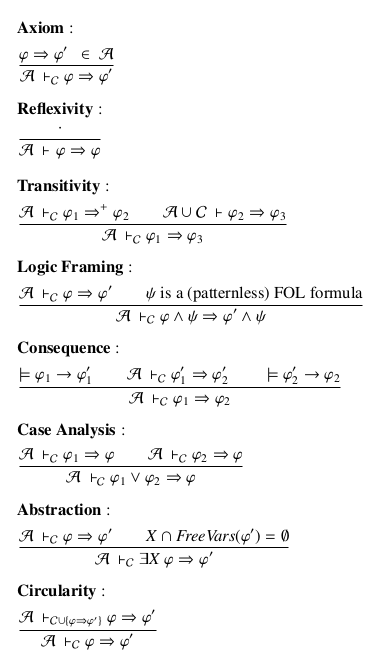
\includegraphics[width=0.5\textwidth]{img/onepath-rl.png}
    \caption{One-path reachability-logic proof system.
    The use of $\Rightarrow^+$ in sequent means that it was derived without Reflexivity.
    TODO retypeset}
    \label{fig:RLproofsystem}
\end{figure}

\begin{lemma}[On equivalence and FOL translation]\label{lem:equivFOLtransl}
    Let $\varphi_1, \varphi_2$ be two matching logic formulas such that $\vDash \varphi_1 \leftrightarrow \varphi_2$.
    Then $\vDash (\varphi_1^\square)[X/\square] \leftrightarrow (\varphi_2^\square)[X/\square]$.
\end{lemma}
\begin{proof}
    Let $M$ be any matching logic model, $\gamma$ an element of $M$, and $\rho$ an $M$-valuation.
    We have to prove that $(M, \gamma, \rho) \vDash (\varphi_1^\square)[X/\square] \leftrightarrow (\varphi_2^\square)[X/\square]$,
    which is (by definition of the squaring function and substitution) equivalent to
    $(M, \gamma, \rho) \vDash ((\varphi_1 \leftrightarrow \varphi_2)^\square)[X/\square]$,
    which is
    (by \Cref{lem:varrenamesem}, because $\rho(X) = \rho[\square := \rho(X)](\square)$)
    equivalent to
    $(M, \gamma, \rho[\square := \rho(X)]) \vDash (\varphi_1 \leftrightarrow \varphi_2)^\square$,
    which is  (by \Cref{lem:patternToFOLSemantics}, because $\rho[\square := \rho(X)] = \rho^{\rho(X)}$) equivalent to
    $(M, \rho(X), \rho) \vDash \varphi_1 \leftrightarrow \varphi_2$,
    which holds by the assumption.
\end{proof}

\begin{proof}[Proof of \Cref{lem:CRLalmostSoundness}]
By induction on the structure of the CRL proof.
\begin{enumerate}
    \item If the proof ends with \emph{Reduce}, then we are done, since $\mathit{flatten}^\exists(\emptyset, \psi^\prime) = \emptyset$.
    
    \item If the proof ends with \emph{Reflexivity}, then we need to prove
    \begin{equation*}
        \mathcal{S}^* \cup \mathit{flatten}^\exists(E, \psi), \emptyset \vdash_\RL
          \mathit{flatten}^\exists(\psi, \psi) 
    \end{equation*}
    which we do by applying the Reflexivity proof rule.
    
    \item If the proof ends with \emph{Axiom}, then $\psi \in E$,
          and we have to prove that
          \begin{equation*}
            \mathcal{S}^* \cup \mathit{flatten}^\prime(E, \psi^\prime), \mathit{flatten}^\prime(C, \psi^\prime) \vdash_\RL
            \mathit{flatten}^\prime(\psi, \psi^\prime)               \, .
          \end{equation*}
          By applying the Axiom proof rule of RL, it is enough to show that
          \begin{equation*}
              \mathit{flatten}^\prime(\psi, \psi^\prime) \in \mathit{flatten^\prime}(E, \psi^\prime) \, ,
          \end{equation*}
          which follows from $\psi \in E$.
          
    \item If the proof ends with \emph{Case}, then we have
        \begin{equation*}
            \mathcal{S}^* \cup \Bar{E}, \Bar{C} \vdash_\RL
            \mathit{flatten}^\exists((\varphi_1, \ldots, \varphi_{i-1}, \varphi_i, \varphi_{i+1}, \ldots, \varphi_k) \land P^\prime, \Psi^\prime)
        \end{equation*}
        and
        \begin{equation*}
            \mathcal{S}^* \cup \Bar{E}, \Bar{C} \vdash_\RL
            \mathit{flatten}^\exists((\varphi_1, \ldots, \varphi_{i-1}, \psi_i, \varphi_{i+1}, \ldots, \varphi_k) \land P^\prime, \Psi^\prime) 
        \end{equation*}
        as hypotheses, and we have to prove
        \begin{equation*}
            \mathcal{S}^* \cup \Bar{E}, \Bar{C} \vdash_\RL
            \mathit{flatten}^\exists((\varphi_1, \ldots, \varphi_{i-1}, (\varphi_i \lor \psi_i), \varphi_{i+1}, \ldots, \varphi_k) \land P^\prime, \Psi^\prime)               \, .
        \end{equation*}
        (where $\Bar{E} = \mathit{flatten}^\exists(E, \psi^\prime)$
         and $\Bar{C} = \mathit{flatten}^\exists(C, \psi^\prime)$
        ).
        After simplifications, we get
        \begin{align*}
            \mathcal{S}^* \cup \Bar{E}, \Bar{C} \vdash_\RL
            &
            \mathit{mkList}(X_1, \ldots, X_k) \land \left( \bigwedge_{j=1}^{k} (\varphi_j^\square)[X_j/\square] \right) \land P^\prime
            \\ & \Rightarrow^\exists
            \mathit{flatten}(\Psi^\prime)
        \end{align*}
        and
        \begin{align*}
            \mathcal{S}^* \cup \Bar{E}, \Bar{C} \vdash_\RL
            &
            \mathit{mkList}(Y_1, \ldots, Y_k) \land \left(\bigwedge_{j=1, j \not = i}^{k} (\varphi_j^\square)[Y_j/\square] \right)
            \land (\psi_i^\square)[Y_i/\square] \land P^\prime
            \\ & \Rightarrow^\exists
            \mathit{flatten}(\Psi^\prime)
        \end{align*}
        as hypotheses,
        and have to prove
        \begin{align*}
            \mathcal{S}^* \cup \Bar{E}, \Bar{C} \vdash_\RL
            &
            \mathit{mkList}(Z_1, \ldots, Z_k) \land \left(\bigwedge_{j=1,j \not = i}^{k} (\varphi_j^\square)[Z_j/\square]\right)
            \land ((\varphi_i \lor \psi_i)^\square)[Z_i/\square]
            \\ & \Rightarrow^\exists
            \mathit{flatten}(\Psi^\prime)
        \end{align*}
        (where $X_1,\ldots,X_k,Y_1,\ldots,Y_k,Z_1,\ldots,Z_k$ are fresh variables).
        We first apply the Consequence RL rule to the goal to distribute the $\varphi_i \lor \psi_i$ disjunction
        to the top, changing the goal to
        \begin{align*}
            \mathcal{S}^* \cup \Bar{E}, \Bar{C} \vdash_\RL
            &
            \left( \mathit{mkList}(Z_1, \ldots, Z_k) \land \left(\bigwedge_{j=1,j \not = i}^{k} (\varphi_j^\square)[Z_j/\square]\right)
            \land (\varphi_i^\square)[Z_i/\square] \right)
            \\ \lor &
            \left(
            \mathit{mkList}(Z_1, \ldots, Z_k) \land \left(\bigwedge_{j=1,j \not = i}^{k} (\varphi_j^\square)[Z_j/\square]\right)
            \land (\psi_i^\square)[Z_i/\square]
            \right)
            \\ & \Rightarrow^\exists
            \mathit{flatten}(\Psi^\prime) \, .
        \end{align*}
        Now we apply the Case Analysis rule.
        Then we transform the hypotheses to the respective goals by existentially quantifying the $X_j$s (and $Y_j$s, respectively)
        in the hypotheses
        using the Abstraction RL rule, alpha-renaming (using the Consequence rule) the $X_j$s (and $Y_j$s, respectively)
        into $Z_j$s, and stripping the existential quantifiers (using the Consequence rule, again), and we are done.
        
    \item If the proof ends with \emph{Step},
      we can assume a structureless FOL formula $P^\prime$, a rule $\varphi \Rightarrow^\exists \varphi^\prime \in S$ such that
      $\mathcal{T} \vDash_\ML \varphi_i \leftrightarrow \varphi \land P^\prime$,
      and an induction hypothesis
      \begin{align*}
        (&\mathcal{T}^*, S^* \cup \mathit{flatten}^\exists(C \cup E, \Psi^\prime)), \emptyset \vdash_\RL
          \\ &
          \mathit{flatten}([\varphi_1, \ldots, \varphi_{i-1}, \varphi^\prime \land P^\prime, \varphi_{i+1}, \ldots, \varphi_k] \land P) \Rightarrow^\exists \mathit{flatten}(\Psi^\prime)     
      \end{align*}
      and have to construct
      \begin{align*}
      & (\mathcal{T}^*, S^* \cup \mathit{flatten}^\exists(E, \Psi^\prime)), \mathit{flatten}^\exists(C, \Psi^\prime) \vdash_\RL \\
          & \mathit{flatten}([\varphi_1, \ldots, \varphi_{i-1}, \varphi_i, \varphi_{i+1}, \ldots, \varphi_k] \land P) \Rightarrow^\exists \mathit{flatten}(\Psi^\prime)    \, .
      \end{align*}
        By definition of $S^*$, we also have
        \begin{align*}
            (\mathit{heat}(L, \varphi, R) \Rightarrow^\exists \mathit{heat}(L, \varphi^\prime, R)) \in S^* \, .
        \end{align*}
    We apply the Transitivity rule with the second premise being our first inductive hypothesis, and it remains to prove the second premise, which is
    \begin{align*}
        & (\mathcal{T}, S)^*, \mathit{flatten}^\exists(E, \psi^\prime), \mathit{flatten}^\exists(C, \psi^\prime)
        \\& \vdash_\RL
        \mathit{flatten}([\varphi_1, \ldots, \varphi_{i-1}, \varphi_i, \varphi_{i+1}, \ldots, \varphi_k] \land P)
        \\&\quad \Rightarrow^\exists
        \mathit{flatten}([\varphi_1, \ldots, \varphi_{i-1}, \varphi^\prime \land P^\prime, \varphi_{i+1}, \ldots, \varphi_k] \land P) \, .
    \end{align*}
    that is (after simplification, assuming a reasonable choice of fresh variables)
    \begin{align*}
        & (\mathcal{T}, S)^*, \mathit{flatten}^\exists(E, \psi^\prime), \mathit{flatten}^\exists(C, \psi^\prime)
        \\& \vdash_\RL
        \mathit{mkList}(X_1, \ldots, X_k) \land \left( \bigwedge_{j=1,j\not = i}^{k} (\varphi_j^\square)[X_j/\square] \right)
        \land (\varphi_i^\square)[X_i/\square] \land P
        \\&\quad \Rightarrow^\exists
        \mathit{mkList}(X_1, \ldots, X_k) \land \left( \bigwedge_{j=1, j \not = i}^{k} (\varphi_j^\square)[X_j/\square] \right) \land ((\varphi^\prime \land P^\prime)^\square)[X_i/\square] \land P
        \, .
    \end{align*}
    By \Cref{lem:equivFOLtransl}, our assumption that $\mathcal{T} \vDash_\ML \varphi_i \leftrightarrow (\varphi \land P^\prime)$,
    and conservativeness,
    we can apply the Consequence rule, and the goal changes to
    \begin{align*}
        & (\mathcal{T}, S)^*, \mathit{flatten}^\exists(E, \psi^\prime), \mathit{flatten}^\exists(C, \psi^\prime)
        \\& \vdash_\RL
        \mathit{mkList}(X_1, \ldots, X_k) \land \left( \bigwedge_{j=1,j\not = i}^{k} (\varphi_j^\square)[X_j/\square] \right)
        \land ((\varphi \land P^\prime)^\square)[X_i/\square] \land P
        \\&\quad \Rightarrow^\exists
        \mathit{mkList}(X_1, \ldots, X_k) \land \left( \bigwedge_{j=1, j \not = i}^{k} (\varphi_j^\square)[X_j/\square] \right) \land ((\varphi^\prime \land P^\prime)^\square)[X_i/\square] \land P
        \, .
    \end{align*}
    We apply the Consequence rule again, changing the goal to
    \begin{align*}
        & (\mathcal{T}, S)^*, \mathit{flatten}^\exists(E, \psi^\prime), \mathit{flatten}^\exists(C, \psi^\prime)
        \\& \vdash_\RL
        (\varphi^\square)[X_i/\square] \land (
        \mathit{mkList}(X_1, \ldots, X_k) \land \left( \bigwedge_{j=1,j\not = i}^{k} (\varphi_j^\square)[X_j/\square] \right)
        \land ((P^\prime)^\square)[X_i/\square] \land P)
        \\&\quad \Rightarrow^\exists
        ((\varphi^\prime)^\square)[X_i/\square] \land (
        \mathit{mkList}(X_1, \ldots, X_k) \land \left( \bigwedge_{j=1, j \not = i}^{k} (\varphi_j^\square)[X_j/\square] \right) \land ((P^\prime)^\square)[X_i/\square] \land P)
        \, .
    \end{align*}
    Now we apply Logic Framing to remove the structureless parts that are the same in both the left and right sides,
    resulting in the goal
    \begin{align*}
        & (\mathcal{T}, S)^*, \mathit{flatten}^\exists(E, \psi^\prime), \mathit{flatten}^\exists(C, \psi^\prime)
        \\& \vdash_\RL
        (\varphi^\square)[X_i/\square] \land
        \mathit{mkList}(X_1, \ldots, X_k)
        \\&\quad \Rightarrow^\exists
        ((\varphi^\prime)^\square)[X_i/\square] \land
        \mathit{mkList}(X_1, \ldots, X_k)
        \, .
    \end{align*}
    Now, from the assumption that $\varphi \Rightarrow^\exists \varphi^\prime \in S$ and the construction of $S^*$
    it follows that
    $\mathit{heat}(L, \varphi, R) \Rightarrow^\exists \mathit{heat}(L, \varphi^\prime, R) \in S^*$;
    and therefore
    $\mathit{cfgheat}(L, \phi, R) \land Q \Rightarrow^\exists \mathit{cfgheat}(L, \phi^\prime, R) \land Q^\prime \in S^*$
    where $\varphi \equiv \phi \land Q$ and $\varphi^\prime \equiv \phi^\prime \land Q^\prime$.
    By semantic reasoning we can prove that
    \begin{align*}
        \mathcal{T}^* \vDash & ((\varphi^\square)[X_i/\square] \land \mathit{mkList}(X_1, \ldots, X_k))
        \\ \leftrightarrow  &
        \mathit{cfgheat}(L, X_i, R)
        \\ & \land L = \mathit{mkList}(X_1, \ldots, X_{i-1})
        \\ & \land R = \mathit{mkList}(X_{i+1}, \ldots, X_k)
        \\ & \land (\phi^\square)[X_i/\square] \land Q
    \end{align*}
    and that
    \begin{align*}
        \mathcal{T}^* \vDash & (((\varphi^\prime)^\square)[X_i/\square] \land \mathit{mkList}(X_1, \ldots, X_k))
        \\ \leftrightarrow  &
        \mathit{cfgheat}(L, X_i, R)
        \\ & \land L = \mathit{mkList}(X_1, \ldots, X_{i-1})
        \\ & \land R = \mathit{mkList}(X_{i+1}, \ldots, X_k)
        \\ & \land ((\phi^\prime)^\square)[X_i/\square] \land Q^\prime \, .
    \end{align*}
    Now we apply Consequence and subsequently strip the $L$,$R$ equalities using Logic Framing, thus getting
    \begin{align*}
        & (\mathcal{T}, S)^*, \mathit{flatten}^\exists(E, \psi^\prime), \mathit{flatten}^\exists(C, \psi^\prime)
        \\& \vdash_\RL
        \mathit{cfgheat}(L, X_i, R) \land (\phi^\square)[X_i/\square] \land Q
        \\&\quad \Rightarrow^\exists
        \mathit{cfgheat}(L, X_i, R) \land ((\phi^\prime)^\square)[X_i/\square] \land Q^\prime
        \, .
    \end{align*}
    Now we use Consequence to expand $\phi^\square$ and $(\phi^\prime)^\square$ into equalities,
    perform the substitution, and use the equalities to replace the $X_i$ subterm of $\mathit{cfgheat}$ with
    $\phi$ and $\phi^\prime$, respectively; this way the goal becomes
    \begin{align*}
        & (\mathcal{T}, S)^*, \mathit{flatten}^\exists(E, \psi^\prime), \mathit{flatten}^\exists(C, \psi^\prime)
        \\& \vdash_\RL
        \mathit{cfgheat}(L, \phi, R) \land Q
        \\&\quad \Rightarrow^\exists
        \mathit{cfgheat}(L, \phi^\prime, R) \land Q^\prime
        \, .
    \end{align*}
    We finish the proof of this case using the Axiom rule.
    
    \item If the proof ends with \emph{Circularity}, we can assume
        \begin{align*}
            (\mathcal{T}^*, S^* \cup \mathit{flatten}^\exists(E, \Psi^\prime)),
            \mathit{flatten}^\exists(C \cup \{ \Psi \}, \Psi^\prime) \vdash_\RL
            \mathit{flatten}^\exists(\Psi, \Psi^\prime)
        \end{align*}
        which simplifies to
        \begin{align*}
            (\mathcal{T}^*, S^* \cup \mathit{flatten}^\exists(E, \Psi^\prime)),
            \mathit{flatten}^\exists(C, \Psi^\prime) \cup \mathit{flatten}^\exists(\{ \Psi \}, \Psi^\prime) \vdash_\RL
            \mathit{flatten}^\exists(\Psi, \Psi^\prime)
        \end{align*}
        and have to prove
        \begin{align*}
            (\mathcal{T}^*, S^* \cup \mathit{flatten}^\exists(E, \Psi^\prime)),
            \mathit{flatten}^\exists(C, \Psi^\prime) \vdash_\RL
            \mathit{flatten}^\exists(\Psi, \Psi^\prime)
        \end{align*}
        which follows from the assumption by Circularity.
        
    \item If the proof ends with \emph{Conseq}, we can assume
    \begin{align*}
        \mathcal{T}^* \vDash_\ML \mathit{flatten}(\Phi) \rightarrow \mathit{flatten}(\Phi^\prime)
    \end{align*}
    and
    \begin{align*}
        (\mathcal{T}^*, S^* \cup \mathit{flatten}^\exists(E, \Psi^\prime)), \mathit{flatten}^\exists(C, \Psi^\prime) \vdash_\RL
          \mathit{flatten}^\exists(\Phi^\prime, \Psi^\prime) \, ,
    \end{align*}
    and have to prove
    \begin{align*}
        (\mathcal{T}^*, S^* \cup \mathit{flatten}^\exists(E, \Psi^\prime)), \mathit{flatten}^\exists(C, \Psi^\prime) \vdash_\RL
          \mathit{flatten}^\exists(\Phi, \Psi^\prime)  \, .
    \end{align*}
    The second assumption simplifies to
    \begin{align*}
        (\mathcal{T}^*, S^* \cup \mathit{flatten}^\exists(E, \Psi^\prime)), \mathit{flatten}^\exists(C, \Psi^\prime) \vdash_\RL
          \mathit{flatten}(\Phi^\prime) \Rightarrow^\exists \mathit{flatten}(\Psi^\prime) \, ,
    \end{align*}
    while the goal to
    \begin{align*}
        (\mathcal{T}^*, S^* \cup \mathit{flatten}^\exists(E, \Psi^\prime)), \mathit{flatten}^\exists(C, \Psi^\prime) \vdash_\RL
          \mathit{flatten}(\Phi) \Rightarrow^\exists \mathit{flatten}(\Psi^\prime) \, ;
    \end{align*}
    therefore, we can apply the \emph{Consequence} rule.        
        
        
    \item If the proof ends with \emph{Abstract},
    we assume
    \begin{align*}
        X \not\in \mathit{FV}(\Psi^\prime)
    \end{align*}
    and
    \begin{align*}
                (\mathcal{T}^*, S^* \cup \mathit{flatten}^\exists(E, \Psi^\prime)), \mathit{flatten}^\exists(C, \Psi^\prime) \vdash_\RL
          \mathit{flatten}^\exists(\exists \vec{Y}.\, (\varphi_1, \ldots, \varphi_k) \land P, \Psi^\prime)
    \end{align*}
    and have to prove that
    \begin{align*}
                (\mathcal{T}^*, S^* \cup \mathit{flatten}^\exists(E, \Psi^\prime)), \mathit{flatten}^\exists(C, \Psi^\prime) \vdash_\RL
          \mathit{flatten}^\exists(\exists X,\vec{Y}.\, (\varphi_1, \ldots, \varphi_k) \land P, \Psi^\prime) \, .
    \end{align*}
    After simplifications, the second premise becomes
    \begin{align*}
            &(\mathcal{T}^*, S^* \cup \mathit{flatten}^\exists(E, \Psi^\prime)), \mathit{flatten}^\exists(C, \Psi^\prime) \vdash_\RL
          \\& \exists \vec{Y}.\, (\mathit{mkList}(Z_1, \ldots, Z_k) \land (\varphi_1^\square)[Z_1/\square] \land \ldots (\varphi_1^\square)[Z_k/\square]) \land P)
          \\&
          \Rightarrow^\exists \mathit{flatten}(\Psi^\prime) \, ,
    \end{align*}
    while the goal becomes
    \begin{align*}
          &(\mathcal{T}^*, S^* \cup \mathit{flatten}^\exists(E, \Psi^\prime)), \mathit{flatten}^\exists(C, \Psi^\prime) \vdash_\RL
          \\&\exists X. \exists \vec{Y}.\, (\mathit{mkList}(Z_1, \ldots, Z_k) \land (\varphi_1^\square)[Z_1/\square] \land \ldots (\varphi_1^\square)[Z_k/\square]) \land P) \, .
    \end{align*}
    We prove the goal using the Abstraction rule
    (note that $X \not\in \mathit{FV}(\Psi^\prime)$ implies $X \not\in \mathit{FV}(\mathit{flatten}(\Psi^\prime))$
    because we are free to choose the fresh variables inside the $\mathit{flatten}$ such).
    \end{enumerate}
    This concludes the proof.
\end{proof}
